\documentclass[12pt,a4paper,oneside]{report}

% ==============================================================================
% 1. CẤU HÌNH GÓI & ĐỊNH NGHĨA KÝ HIỆU TOÁN
% ==============================================================================
% ==============================================================================
% CẤU HÌNH HỆ THỐNG & PREAMBLE CHUẨN ĐỒ ÁN
% Tương thích hoàn hảo với cả XeLaTeX (khuyên dùng trên macOS) và pdfLaTeX
% ==============================================================================
\usepackage{iftex}

\ifXeTeX
  \usepackage{fontspec}
  \setmainfont{Times New Roman}
\else
  \usepackage[utf8]{inputenc}
  \usepackage[T5,T1]{fontenc}
\fi

% ==============================================================================
% 1. VIỆT HÓA CÁC TIÊU ĐỀ MẶC ĐỊNH
% ==============================================================================
\newcommand{\chaptertitlename}{Chương}
\renewcommand{\contentsname}{Mục lục}
\renewcommand{\listfigurename}{Danh mục hình vẽ}
\renewcommand{\listtablename}{Danh mục bảng biểu}
\renewcommand{\bibname}{Tài liệu tham khảo}
\renewcommand{\figurename}{Hình}
\renewcommand{\tablename}{Bảng}

% ==============================================================================
% 2. CĂN LỀ CHUẨN ĐỒ ÁN / BÁO CÁO KHOA HỌC
%    Top: 2.5cm | Bottom: 2.5cm | Left: 3.5cm (đóng gáy) | Right: 2.0cm
% ==============================================================================
\usepackage{geometry}
\geometry{
    a4paper,
    top=25mm,
    bottom=25mm,
    left=35mm,
    right=20mm,
    includehead,
    includefoot
}

% Giãn dòng chuẩn 1.3 & thụt lề
\usepackage{setspace}
\setstretch{1.3}
\setlength{\parindent}{1cm}
\setlength{\parskip}{6pt}

% ==============================================================================
% 3. GÓI TOÁN HỌC & HÌNH ẢNH
% ==============================================================================
\usepackage{amsmath,amssymb,amsthm}
\usepackage{graphicx}
\graphicspath{{figures/}} % Đường dẫn đến thư mục hình ảnh
\usepackage{xcolor}
\usepackage{tikz}
\usetikzlibrary{arrows.meta, positioning, calc}
\usepackage{booktabs}
\usepackage{array}

% ==============================================================================
% 4. ĐỊNH DẠNG TIÊU ĐỀ CHƯƠNG CHUẨN (KHÔNG CẦN CÀI THÊM GÓI PHỤ)
% ==============================================================================
\makeatletter
\def\@makechapterhead#1{%
  \vspace*{5\p@}%
  {\parindent \z@ \centering \normalfont
    \ifnum \c@secnumdepth >\m@ne
      \large\bfseries \MakeUppercase{\chaptertitlename}\ \thechapter
      \par\nobreak
      \vskip 8\p@
    \fi
    \interlinepenalty\@M
    \LARGE \bfseries \MakeUppercase{#1}\par\nobreak
    \vskip 22\p@
  }}
\def\@makeschapterhead#1{%
  \vspace*{5\p@}%
  {\parindent \z@ \centering \normalfont
    \interlinepenalty\@M
    \LARGE \bfseries \MakeUppercase{#1}\par\nobreak
    \vskip 22\p@
  }}
\makeatother

% ==============================================================================
% 5. ĐỊNH DẠNG MÔI TRƯỜNG ĐỊNH LÝ / BỔ ĐỀ / BÀI TẬP
% ==============================================================================
\theoremstyle{plain}
\newtheorem{theorem}{Định lý}[chapter]
\newtheorem{lemma}[theorem]{Bổ đề}
\newtheorem{corollary}[theorem]{Hệ quả}
\newtheorem{proposition}[theorem]{Mệnh đề}

\theoremstyle{definition}
\newtheorem{definition}[theorem]{Định nghĩa}
\newtheorem{example}[theorem]{Ví dụ}
\newtheorem{exercise}{Bài tập}[chapter]

\theoremstyle{remark}
\newtheorem{remark}[theorem]{Nhận xét}

\renewcommand{\qedsymbol}{$\blacksquare$}

% ==============================================================================
% 6. HEADER & FOOTER (FANCYHDR)
% ==============================================================================
\usepackage{fancyhdr}
\pagestyle{fancy}
\fancyhf{}
\setlength{\headheight}{15pt}
\fancyhead[L]{\small\slshape Đề tài 5: Khôi phục tín hiệu thưa}
\fancyhead[R]{\small\slshape\nouppercase{\leftmark}}
\fancyfoot[C]{\thepage}
\renewcommand{\headrulewidth}{0.5pt}
\renewcommand{\footrulewidth}{0.3pt}

% Trang đầu chương không hiện header
\fancypagestyle{plain}{
    \fancyhf{}
    \fancyfoot[C]{\thepage}
    \renewcommand{\headrulewidth}{0pt}
    \renewcommand{\footrulewidth}{0pt}
}

% ==============================================================================
% 7. HYPERLINK & BOOKMARK
% ==============================================================================
\usepackage[
    colorlinks=true,
    linkcolor=blue!75!black,
    citecolor=teal!80!black,
    urlcolor=blue!60!black,
    bookmarksnumbered=true,
    pdfstartview=FitH
]{hyperref}
\usepackage{bookmark}

% ==============================================================================
% CÁC MACRO VÀ KÝ HIỆU TOÁN HỌC DÙNG CHUNG
% ==============================================================================

% Ký hiệu định nghĩa (coloneqq) an toàn
\providecommand{\coloneqq}{\mathrel{\mathop:}=}

% Tập hợp số
\newcommand{\R}{\mathbb{R}}
\newcommand{\N}{\mathbb{N}}
\newcommand{\Z}{\mathbb{Z}}
\newcommand{\C}{\mathbb{C}}

% Toán tử toán học
\DeclareMathOperator{\supp}{supp}
\DeclareMathOperator{\spark}{spark}
\DeclareMathOperator{\sign}{sign}
\DeclareMathOperator{\argmin}{arg\,min}
\DeclareMathOperator{\argmax}{arg\,max}
\DeclareMathOperator{\diag}{diag}
\DeclareMathOperator{\rank}{rank}

% Ký hiệu chuẩn và tích vô hướng thuận tiện
\newcommand{\normzero}[1]{\|#1\|_0}
\newcommand{\normone}[1]{\|#1\|_1}
\newcommand{\normtwo}[1]{\|#1\|_2}
\newcommand{\inner}[2]{\langle #1, #2 \rangle}


\begin{document}

% ------------------------------------------------------------------------------
% 2. CÁC TRANG ĐẦU (FRONTMATTER: BÌA, LỜI MỞ ĐẦU, MỤC LỤC)
% ------------------------------------------------------------------------------
\pagenumbering{roman}

% Trang bìa chính
% ==============================================================================
% TRANG BÌA CHUẨN ĐỒ ÁN - ĐẠI HỌC GIAO THÔNG VẬN TẢI
% Gồm 2 bìa: Bìa chính (không có tên thành viên) và Bìa phụ (có tên thành viên)
% ==============================================================================

\newcommand{\drawcoverborder}{%
    \begin{tikzpicture}[remember picture, overlay]
        \coordinate (NW) at ($(current page.north west) + (22mm, -18mm)$);
        \coordinate (SE) at ($(current page.south east) + (-16mm, 18mm)$);
        \coordinate (NE) at ($(current page.north east) + (-16mm, -18mm)$);
        \coordinate (SW) at ($(current page.south west) + (22mm, 18mm)$);
        
        % Khung ngoài (màu đen thanh mảnh)
        \draw[line width=1pt, black] (NW) rectangle (SE);
        
        % Khung viền trong (màu đỏ đậm nổi bật)
        \draw[line width=2pt, red!80!black] 
            ($(NW) + (2.2mm, -2.2mm)$) rectangle ($(SE) + (-2.2mm, 2.2mm)$);
            
        % Khung viền trong cùng (đường chỉ đen mảnh)
        \draw[line width=0.6pt, black] 
            ($(NW) + (3.6mm, -3.6mm)$) rectangle ($(SE) + (-3.6mm, 3.6mm)$);
            
        % Họa tiết 4 góc vuông giao nhau
        \foreach \corner in {NW, NE, SW, SE} {
            \draw[line width=0.8pt, black, fill=white] 
                ($(\corner) + (-3mm, -3mm)$) rectangle ($(\corner) + (3mm, 3mm)$);
            \draw[line width=0.5pt, red!80!black] 
                ($(\corner) + (-1.8mm, -1.8mm)$) rectangle ($(\corner) + (1.8mm, 1.8mm)$);
        }
    \end{tikzpicture}%
}

% ------------------------------------------------------------------------------
% 1. BÌA CHÍNH (Không có danh sách thành viên)
% ------------------------------------------------------------------------------
\begin{titlepage}
    \drawcoverborder
    \centering
    \vspace*{-0.6cm}

    {\fontsize{13pt}{16pt}\selectfont\bfseries TRƯỜNG ĐẠI HỌC GIAO THÔNG VẬN TẢI\par}
    \vspace{0.15cm}
    {\fontsize{13pt}{16pt}\selectfont\bfseries KHOA CÔNG NGHỆ THÔNG TIN\par}
    
    \vspace{1.2cm}
    
\includegraphics[width=3.4cm, height=3.4cm, keepaspectratio]{logo_utc.jpg}
    \vspace{1.2cm}

    {\fontsize{18pt}{22pt}\selectfont\bfseries ĐỒ ÁN MÔN\par}
    \vspace{1.0cm}

    {\fontsize{15pt}{21pt}\selectfont\bfseries TÌM HIỂU BÀI TOÁN KHÔI PHỤC TÍN HIỆU THƯA\\BẰNG CỰC TIỂU HÓA CHUẨN $\ell_1$\par}

    \vfill
    {\fontsize{12pt}{15pt}\selectfont\bfseries HÀ NỘI, T11/2026\par}
    \vspace*{0.6cm}
\end{titlepage}

% ------------------------------------------------------------------------------
% 2. BÌA PHỤ (Có danh sách thành viên và Giảng viên hướng dẫn)
% ------------------------------------------------------------------------------
\begin{titlepage}
    \drawcoverborder
    \centering
    \vspace*{-0.8cm}

    {\fontsize{13pt}{16pt}\selectfont\bfseries TRƯỜNG ĐẠI HỌC GIAO THÔNG VẬN TẢI\par}
    \vspace{0.1cm}
    {\fontsize{13pt}{16pt}\selectfont\bfseries KHOA CÔNG NGHỆ THÔNG TIN\par}
    
    \vspace{0.4cm}
    
\includegraphics[width=3.0cm, height=3.0cm, keepaspectratio]{logo_utc.jpg}
    \vspace{0.4cm}

    {\fontsize{16pt}{20pt}\selectfont\bfseries ĐỒ ÁN MÔN\par}
    \vspace{0.4cm}

    {\fontsize{14pt}{19pt}\selectfont\bfseries TÌM HIỂU BÀI TOÁN KHÔI PHỤC TÍN HIỆU THƯA\\BẰNG CỰC TIỂU HÓA CHUẨN $\ell_1$\par}

    \vspace{0.7cm}

    \begin{flushleft}
        \hspace*{1.0cm}
        \begin{tabular}{rll}
            \textbf{Sinh viên thực hiện:} 
            & Nguyễn Thị Hạnh      & \quad 233000575 \\[0.08cm]
            & Bùi Doãn Mạnh        & \quad 233030594 \\[0.08cm]
            & Hoàng Quốc Duy       & \quad 233030559 \\[0.08cm]
            & Phạm Quang Tài       & \quad 233030608 \\[0.08cm]
            & Đoàn Văn Bảo         & \quad 233030554 \\[0.08cm]
            & Nguyễn Bùi Quang Huy & \quad 233030583 \\[0.08cm]
            & Nguyễn Quang Duy     & \quad 233030561 \\[0.08cm]
            & Phạm Đức Tuấn Hùng   & \quad 233030582 \\[0.30cm]
            \textbf{Giảng viên hướng dẫn:} 
            & \multicolumn{2}{l}{Nguyễn Thế Vinh}
        \end{tabular}
    \end{flushleft}

    \vfill
    {\fontsize{12pt}{15pt}\selectfont\bfseries HÀ NỘI, T11/2026\par}
    \vspace*{0.6cm}
\end{titlepage}


% Lời mở đầu / tóm tắt đề tài
% ==============================================================================
% LỜI MỞ ĐẦU & TÓM TẮT ĐỀ TÀI
% ==============================================================================
\chapter*{Lời mở đầu}
\addcontentsline{toc}{chapter}{Lời mở đầu}

Trong thời đại số hóa, khối lượng dữ liệu được thu thập từ các hệ thống cảm biến, thiết bị chẩn đoán y tế, viễn thông và thị giác máy tính ngày càng tăng với tốc độ bùng nổ. Tuy nhiên, việc thu nhận toàn bộ các thành phần của tín hiệu thường vấp phải các rào cản vật lý nghiêm ngặt: giới hạn về thời gian quét của máy chụp ảnh cộng hưởng từ (MRI), giới hạn năng lượng pin của các cảm biến không dây, hoặc hạn chế về băng thông truyền dẫn trong mạng viễn thông.

Thách thức trung tâm của bài toán đặt ra là: \emph{Làm thế nào để khôi phục chính xác tín hiệu ban đầu khi số phép đo thực tế ít hơn rất nhiều so với số chiều của tín hiệu, đồng thời dữ liệu lại chịu ảnh hưởng của nhiễu ngẫu nhiên?}

Thông qua lý thuyết Lấy mẫu nén (\emph{Compressed Sensing}), tính chất thưa (\emph{sparsity}) đóng vai trò là chiếc chìa khóa quyết định. Việc tối ưu hóa chuẩn $\ell_1$ cho phép chuyển bài toán đếm tổ hợp NP-hard sang bài toán quy hoạch lồi giải được trong thời gian đa thức.

Đồ án này tập trung vào 4 trọng tâm nghiên cứu:
\begin{enumerate}
    \item Hệ thống hóa cơ sở toán học và các mô hình tối ưu chuẩn: Basis Pursuit (BP), Basis Pursuit Denoising (BPDN) và LASSO.
    \item Phân tích các điều kiện khôi phục lý thuyết cốt lõi: Spark, Tính chất không gian hạt nhân (NSP), Tính tương quan qua lại (Mutual Coherence) và Tính chất đẳng cự hạn chế (RIP).
    \item Cài đặt và đánh giá các thuật toán tối ưu bậc nhất: ISTA, FISTA, GPSR và thuật toán nhân tử Lagrange tăng cường ADMM.
    \item Xây dựng quy trình thực nghiệm mô phỏng và kiểm chứng trên ảnh thực tế.
\end{enumerate}

\clearpage

% Mục lục & Danh mục hình vẽ, bảng biểu (cỡ chữ và khoảng cách cân đối, đều nhau)
{
\small
\setstretch{1.05}
\setlength{\parskip}{2pt}
\makeatletter
\renewcommand*\l@chapter[2]{%
  \ifnum \c@tocdepth >\m@ne
    \addpenalty{-\@highpenalty}%
    \vskip 0.55em \@plus\p@
    \setlength\@tempdima{1.5em}%
    \begingroup
      \parindent \z@ \rightskip \@pnumwidth
      \parfillskip -\@pnumwidth
      \leavevmode \bfseries
      \advance\leftskip\@tempdima
      \hskip -\leftskip
      #1\nobreak\hfil \nobreak\hb@xt@\@pnumwidth{\hss #2}\par
      \penalty\@highpenalty
    \endgroup
  \fi}
\makeatother
\tableofcontents
\clearpage

\begingroup
\renewcommand{\addvspace}[1]{\vspace{3pt}}
\phantomsection
\addcontentsline{toc}{chapter}{Danh mục hình vẽ}
\listoffigures
\clearpage

\phantomsection
\addcontentsline{toc}{chapter}{Danh mục bảng biểu}
\listoftables
\clearpage
\endgroup
}

% ------------------------------------------------------------------------------
% 3. NỘI DUNG CHÍNH (MAINMATTER: CÁC CHƯƠNG)
% ------------------------------------------------------------------------------
\pagenumbering{arabic}
\setcounter{page}{1}

% Chương 1: Tổng quan và cơ sở về tín hiệu thưa
% ==============================================================================
% CHƯƠNG 1: TỔNG QUAN VÀ CƠ SỞ VỀ TÍN HIỆU THƯA
% ==============================================================================
\chapter{Tổng quan và cơ sở về tín hiệu thưa}
\label{chap:tong_quan}

\section{Đặt vấn đề và động lực nghiên cứu}
Trong thời đại bùng nổ dữ liệu số, việc thu thập, lưu trữ và truyền tải thông tin đối mặt với những thách thức vật lý to lớn. Theo định lý lấy mẫu cổ điển Shannon--Nyquist, để tái tạo một tín hiệu liên tục có dải tần giới hạn bởi tần số cực đại $f_{\max}$, tần số lấy mẫu tối thiểu phải thỏa mãn điều kiện $f_s \ge 2 f_{\max}$. Tuy nhiên, trong nhiều ứng dụng hiện đại:
\begin{itemize}
    \item \textbf{Chụp ảnh cộng hưởng từ (MRI):} Việc lấy mẫu toàn phần đòi hỏi bệnh nhân phải nằm yên trong máy quét hàng giờ, gây khó chịu và dễ tạo ra hiện tượng nhòe ảnh do cử động sinh học. Giảm số lượng phép đo là yêu cầu sống còn để rút ngắn thời gian quét.
    \item \textbf{Mạng cảm biến không dây (Wireless Sensor Networks):} Các nút cảm biến hoạt động bằng pin năng lượng hữu hạn trong điều kiện khắc nghiệt. Việc truyền tải dữ liệu tiêu hao tới 80\% năng lượng của nút; do đó, nén dữ liệu ngay tại khâu đo lường giúp kéo dài tuổi thọ mạng.
    \item \textbf{Hệ thống viễn thông và radar mảng pha:} Băng thông truyền thông và tốc độ chuyển đổi tương tự--số (ADC) luôn bị giới hạn bởi phần cứng vật lý.
\end{itemize}

Bài toán cốt lõi đặt ra là: \emph{Từ một số lượng rất ít các phép đo gián tiếp và có thể bị nhiễu, liệu ta có thể tái tạo chính xác tín hiệu ban đầu?}

Mô hình toán học dẫn đến hệ phương trình đại số tuyến tính:
\begin{equation}
    Ax = b,
    \label{eq:underdetermined_system}
\end{equation}
trong đó:
\begin{itemize}
    \item $x \in \R^n$ là vector biểu diễn tín hiệu nguyên bản cần tìm.
    \item $A \in \R^{m \times n}$ là ma trận đo lường tuyến tính với $m < n$ (thậm chí $m \ll n$).
    \item $b \in \R^m$ là vector quan sát (kết quả phép đo).
\end{itemize}

Về mặt đại số tuyến tính thuần túy, ma trận $A$ có số cột nhiều hơn số hàng ($m < n$), do đó không gian hạt nhân $\ker(A) \coloneqq \{h \in \R^n : Ah = 0\}$ có số chiều ít nhất là $n - m > 0$. Nếu hệ có một nghiệm $x_0$, thì toàn bộ không gian affine $x_0 + \ker(A)$ gồm vô số phần tử đều là nghiệm của \eqref{eq:underdetermined_system}. 

Tuy nhiên, nếu ta biết thêm thông tin cấu trúc tiên nghiệm: \textbf{tín hiệu thực sự mang thông tin là một tín hiệu thưa} (hầu hết các tọa độ bằng 0), thì giao điểm giữa tập hợp các vector thưa và không gian nghiệm affine $x_0 + \ker(A)$ hoàn toàn có thể là một điểm duy nhất. Lý thuyết Lấy mẫu nén (\emph{Compressed Sensing}) khẳng định rằng: thông tin cấu trúc này cho phép giải quyết trọn vẹn nghịch lý thiếu phương trình.

\section{Tín hiệu và biểu diễn thưa trong cơ sở biến đổi}
Tín hiệu trong tự nhiên ban đầu là các hàm liên tục: âm thanh $s(t)$, ảnh số $I(u, v)$, hoặc video $V(u, v, t)$. Khi số hóa, ta lấy mẫu tín hiệu liên tục tại các thời điểm rời rạc $t_j = j T_s$, tạo thành dãy $\{x_j\}$, tương ứng với vector $x \in \R^n$. Một bức ảnh có kích thước $p \times q$ cũng có thể vector hóa thành một phần tử trong không gian $\R^{pq}$.

\begin{figure}[htbp]
    \centering
    \begin{tikzpicture}[>=stealth, auto, node distance=2.5cm,
        block/.style={rectangle, draw=blue!70!black, fill=blue!5, thick, rounded corners, minimum height=3em, minimum width=6.5em, text centered}]
        
        \node [block] (a) {Tín hiệu $s(t)$};
        \node [block, right=2.5cm of a] (b) {Vector $x \in \R^n$};
        \node [block, right=2.5cm of b] (c) {Phép đo $b = Ax + e$};
        
        \draw [->, thick] (a) -- node [above] {Lấy mẫu} (b);
        \draw [->, thick] (b) -- node [above] {Đo nén} (c);
    \end{tikzpicture}
    \caption{Sơ đồ chuỗi biến đổi từ tín hiệu liên tục, qua số hóa rời rạc đến phép đo nén tuyến tính có nhiễu.}
    \label{fig:sampling_process}
\end{figure}

Phép đo nén $b_i = \sum_{j=1}^n a_{ij} x_j + e_i$ thu nhận sự kết hợp tuyến tính toàn cục từ các tọa độ của tín hiệu, không phải là việc ngẫu nhiên chọn lấy một vài thành phần đơn lẻ của $x$.

Trong nhiều bài toán thực tế, tín hiệu $x$ không thưa trực tiếp trong miền thời gian hay không gian gốc, nhưng có biểu diễn thưa thông qua một cơ sở trực chuẩn hoặc từ điển $\Psi \in \R^{n \times n}$ (chẳng hạn như biến đổi Fourier rời rạc DFT hoặc Wavelet):
\begin{equation}
    x = \Psi \theta = \sum_{j=1}^n \theta_j \psi_j,
\end{equation}
trong đó $\theta \in \R^n$ là vector hệ số thưa. Khi đó phương trình đo trở thành:
\begin{equation}
    b = A x + e = A \Psi \theta + e = \widetilde{A} \theta + e,
\end{equation}
với $\widetilde{A} \coloneqq A \Psi \in \R^{m \times n}$ đóng vai trò là ma trận đo tương đương. Sau khi giải tìm được $\theta$, tín hiệu gốc được khôi phục chính xác thông qua phép tổng hợp $x = \Psi \theta$.

\section{Chuẩn và khái niệm thưa toán học}
\begin{definition}[Các chuẩn và đại lượng đếm]
Cho vector $x = (x_1, \dots, x_n)^T \in \R^n$. Ta định nghĩa:
\begin{itemize}
    \item ``Chuẩn'' $\ell_0$ (đếm số tọa độ khác 0):
    \[
    \normzero{x} \coloneqq \#\{i \in \{1, \dots, n\} : x_i \ne 0\}.
    \]
    \item Chuẩn $\ell_1$ (chuẩn tổng giá trị tuyệt đối):
    \[
    \normone{x} \coloneqq \sum_{i=1}^n |x_i|.
    \]
    \item Chuẩn $\ell_2$ (chuẩn khoảng cách Euclid):
    \[
    \normtwo{x} \coloneqq \left( \sum_{i=1}^n x_i^2 \right)^{1/2}.
    \]
\end{itemize}
\end{definition}

\begin{remark}[Bản chất phi chuẩn của $\ell_0$]
Đại lượng $\normzero{x}$ không phải là một chuẩn toán học thực sự vì nó vi phạm tính chất thuần nhất tuyệt đối: với mọi hằng số vô hướng $\alpha \ne 0, 1$, ta có:
\[
\normzero{\alpha x} = \normzero{x} \ne |\alpha| \normzero{x}.
\]
Ngoài ra, $\normzero{\cdot}$ không phải là một hàm lồi (ví dụ: với $x = (1, 0)^T, y = (0, 1)^T$, ta có $\normzero{x} = 1, \normzero{y} = 1$, nhưng $\normzero{\frac{1}{2}x + \frac{1}{2}y} = \normzero{(0.5, 0.5)^T} = 2 > \frac{1}{2}\normzero{x} + \frac{1}{2}\normzero{y} = 1$).
\end{remark}

Vector $x \in \R^n$ được gọi là \textbf{$k$-thưa} ($k$-sparse) nếu số lượng thành phần khác không của nó không vượt quá $k$:
\[
\normzero{x} \le k.
\]
Tập hợp các chỉ số khác không của $x$ được gọi là \textbf{tập hỗ trợ} (\emph{support}):
\begin{equation}
    \supp(x) \coloneqq \{i \in \{1, \dots, n\} : x_i \ne 0\}, \quad |\supp(x)| = \normzero{x}.
\end{equation}

\begin{lemma}[Bất đẳng thức kép giữa chuẩn $\ell_1$ và $\ell_2$]
Với mọi $x \in \R^n$, ta có bất đẳng thức kép:
\begin{equation}
    \normtwo{x} \le \normone{x} \le \sqrt{n} \normtwo{x}.
    \label{eq:norm_inequality}
\end{equation}
Dấu bằng ở vế trái xảy ra khi và chỉ khi $x$ là $1$-thưa (chỉ có tối đa một tọa độ khác không). Dấu bằng ở vế phải xảy ra khi và chỉ khi tất cả các tọa độ có cùng trị tuyệt đối ($|x_1| = |x_2| = \dots = |x_n|$).
\end{lemma}

\begin{proof}
Để chứng minh vế trái $\normtwo{x} \le \normone{x}$, ta tính bình phương của chuẩn $\ell_1$:
\[
\normone{x}^2 = \left( \sum_{i=1}^n |x_i| \right)^2 = \sum_{i=1}^n |x_i|^2 + 2\sum_{1 \le i < j \le n} |x_i| |x_j| = \normtwo{x}^2 + 2\sum_{i < j} |x_i| |x_j|.
\]
Do tích $|x_i| |x_j| \ge 0$, ta có $\normone{x}^2 \ge \normtwo{x}^2$. Lấy căn bậc hai hai vế không âm, ta thu được $\normone{x} \ge \normtwo{x}$. Dấu bằng xảy ra khi và chỉ khi $\sum_{i < j} |x_i| |x_j| = 0$, nghĩa là không thể có đồng thời hai tọa độ khác không ($x$ là $1$-thưa).

Để chứng minh vế phải $\normone{x} \le \sqrt{n} \normtwo{x}$, áp dụng bất đẳng thức Cauchy--Schwarz cho hai vector $u = (|x_1|, \dots, |x_n|)^T$ và $v = (1, \dots, 1)^T \in \R^n$:
\[
\normone{x} = \sum_{i=1}^n |x_i| \cdot 1 = \langle u, v \rangle \le \normtwo{u} \normtwo{v} = \sqrt{\sum_{i=1}^n |x_i|^2} \cdot \sqrt{\sum_{i=1}^n 1^2} = \sqrt{n} \normtwo{x}.
\]
Dấu bằng xảy ra khi và chỉ khi $u$ tỷ lệ với $v$, tức $|x_1| = |x_2| = \dots = |x_n|$.
\end{proof}

\section{Tính thưa xấp xỉ và sai số xấp xỉ tốt nhất}
Trong thực tế, do nhiễu và bản chất liên tục của thế giới thực, các tín hiệu vật lý hiếm khi có các tọa độ bằng 0 chính xác tuyệt đối, mà thường có dạng \textbf{thưa xấp xỉ} (\emph{approximately sparse} hay \emph{compressible}): gồm một số ít hệ số lớn mang phần lớn năng lượng, và rất nhiều hệ số nhỏ suy giảm nhanh về 0 (tuân theo quy luật lũy thừa).

Sai số xấp xỉ $k$-thưa tốt nhất của vector $x$ theo chuẩn $\ell_1$ được định nghĩa là:
\begin{equation}
    \sigma_k(x)_1 \coloneqq \inf_{\normzero{z} \le k} \normone{x - z}.
    \label{eq:best_k_term_approx}
\end{equation}

\begin{exercise}[Chứng minh bài toán xấp xỉ tốt nhất của thầy]
Chứng minh rằng infimum trong \eqref{eq:best_k_term_approx} đạt được tại vector $z^*$ tạo bởi việc giữ lại đúng $k$ tọa độ có giá trị tuyệt đối lớn nhất của $x$ và gán tất cả các tọa độ còn lại bằng 0.
\end{exercise}

\begin{proof}[Lời giải chi tiết của sinh viên]
Giả sử vector $x \in \R^n$ có các tọa độ được sắp xếp theo thứ tự giảm dần của trị tuyệt đối:
\[
|x_{\pi(1)}| \ge |x_{\pi(2)}| \ge \dots \ge |x_{\pi(k)}| \ge |x_{\pi(k+1)}| \ge \dots \ge |x_{\pi(n)}|,
\]
với $\pi$ là một hoán vị của tập chỉ số $\{1, 2, \dots, n\}$. Đặt $S = \{\pi(1), \pi(2), \dots, \pi(k)\}$, với $|S| = k$. 
Định nghĩa vector $z^* \in \R^n$ như sau:
\[
z^*_i = 
\begin{cases}
x_i, & \text{nếu } i \in S, \\
0, & \text{nếu } i \notin S.
\end{cases}
\]
Rõ ràng $\normzero{z^*} = |S| = k$, do đó $z^*$ là một ứng viên khả thi. Khi đó:
\[
\normone{x - z^*} = \sum_{i \in S} |x_i - x_i| + \sum_{i \notin S} |x_i - 0| = \sum_{j=k+1}^n |x_{\pi(j)}|.
\]

Bây giờ xét một vector $k$-thưa tùy ý $z \in \R^n$ với tập hỗ trợ $T = \supp(z)$, thỏa mãn $|T| \le k$.
Sử dụng tính chất phân tách của chuẩn $\ell_1$:
\[
\normone{x - z} = \sum_{i \in T} |x_i - z_i| + \sum_{i \notin T} |x_i - 0| \ge \sum_{i \notin T} |x_i|.
\]
Tập hợp $\{1, \dots, n\} \setminus T$ có lực lượng ít nhất là $n - k$. Do $S$ là tập hợp gồm $k$ phần tử có giá trị tuyệt đối lớn nhất của $x$, tập hợp bù $S^c$ chính là tập hợp gồm $n - k$ phần tử có giá trị tuyệt đối nhỏ nhất. Do đó, tổng trên tập bù của bất kỳ tập $T$ nào có kích thước không quá $k$ đều không nhỏ hơn tổng trên $S^c$:
\[
\sum_{i \notin T} |x_i| \ge \sum_{i \in S^c} |x_i| = \sum_{j=k+1}^n |x_{\pi(j)}| = \normone{x - z^*}.
\]
Như vậy, với mọi vector $k$-thưa $z$, ta luôn có $\normone{x - z} \ge \normone{x - z^*}$. Do đó:
\[
\sigma_k(x)_1 = \normone{x - z^*} = \sum_{j=k+1}^n |x_{\pi(j)}|.
\]
Bài tập được chứng minh trọn vẹn.
\end{proof}


% Chương 2: Các mô hình tối ưu và hình học của chuẩn l1
% ==============================================================================
% CHƯƠNG 2: CÁC MÔ HÌNH TỐI ƯU VÀ HÌNH HỌC CHUẨN L1
% ==============================================================================
\chapter{Các mô hình tối ưu và hình học của chuẩn $\ell_1$}
\label{chap:mo_hinh_toi_uu}

\section{Hệ thống các mô hình tối ưu khôi phục tín hiệu}
Xét bài toán quan sát tuyến tính:
\begin{equation}
    b = A x^\natural + e,
\end{equation}
trong đó $x^\natural \in \R^n$ là tín hiệu nguyên bản cần tìm, ma trận đo $A \in \R^{m \times n}$ ($m < n$), và $e \in \R^m$ là vector nhiễu.

\subsection{Bài toán cực tiểu hóa chuẩn $\ell_0$ và tính bất khả triệt NP-hard}
Trong trường hợp lý tưởng không có nhiễu ($e = 0$), bài toán trực tiếp nhất là tìm kiếm vector có số phần tử khác không ít nhất thỏa mãn các phương trình đo:
\begin{equation}
    (P_0) \quad \min_{x \in \R^n} \normzero{x} \quad \text{s.t.} \quad Ax = b.
\end{equation}

Mặc dù mô hình $(P_0)$ phản ánh đúng định nghĩa của tính thưa, bài toán này thuộc lớp \textbf{NP-hard} (đã được chứng minh bởi Natarajan, 1995). Về mặt tổ hợp, để giải $(P_0)$, ta phải duyệt qua tất cả các tổ hợp gồm $k$ cột trong số $n$ cột của ma trận $A$, tức $\binom{n}{k}$ không gian con. Khi $n$ và $k$ chỉ ở mức trung bình (ví dụ $n = 500, k = 30$), số lượng tổ hợp là $\binom{500}{30} \approx 1{,}4 \times 10^{48}$, vượt quá khả năng tính toán của mọi siêu máy tính. Hơn nữa, hàm mục tiêu $\normzero{\cdot}$ gián đoạn và không lồi, khiến mọi phương pháp giải tích dựa trên đạo hàm hoàn toàn vô hiệu.

\begin{theorem}[Tính lồi của chuẩn $\ell_1$ và không lồi của $\ell_0$]
Chuẩn $\normone{\cdot}$ là một hàm lồi trên $\R^n$, trong khi đại lượng $\normzero{\cdot}$ không phải là hàm lồi.
\end{theorem}

\begin{proof}
1. \textbf{Tính lồi của chuẩn $\ell_1$:} Với mọi $x, y \in \R^n$ và mọi $\alpha \in [0, 1]$, theo bất đẳng thức tam giác của giá trị tuyệt đối:
\[
\normone{\alpha x + (1 - \alpha) y} = \sum_{i=1}^n |\alpha x_i + (1 - \alpha) y_i| \le \sum_{i=1}^n \left( \alpha |x_i| + (1 - \alpha) |y_i| \right) = \alpha \normone{x} + (1 - \alpha) \normone{y}.
\]
Do đó hàm chuẩn $\ell_1$ là hàm lồi (nhưng không lồi ngặt, vì nó tuyến tính trên từng góc phần tư).

2. \textbf{Tính không lồi của chuẩn $\ell_0$:} Ta chứng minh bằng một phản ví dụ trong $\R^2$. Chọn $x = (2, 0)^T$ và $y = (0, 2)^T$. Ta có $\normzero{x} = 1$ và $\normzero{y} = 1$. Chọn $\alpha = \frac{1}{2}$, khi đó:
\[
z = \frac{1}{2}x + \frac{1}{2}y = (1, 1)^T \implies \normzero{z} = 2.
\]
Tuy nhiên:
\[
\alpha \normzero{x} + (1 - \alpha) \normzero{y} = \frac{1}{2}(1) + \frac{1}{2}(1) = 1.
\]
Vì $\normzero{z} = 2 > 1$, hàm $\normzero{\cdot}$ không thỏa mãn định nghĩa hàm lồi.
\end{proof}

\subsection{Bài toán Basis Pursuit (BP)}
Kỹ thuật giải tỏa lồi (\emph{convex relaxation}) thay thế hàm $\normzero{\cdot}$ bằng bao lồi (\emph{convex envelope}) của nó trên hình hộp $\{x : \|x\|_\infty \le 1\}$, chính là chuẩn $\ell_1$, đưa về bài toán \textbf{Basis Pursuit (BP)} \cite{donoho2006compressed, foucart2013mathematical}:
\begin{equation}
    (BP) \quad \min_{x \in \R^n} \normone{x} \quad \text{s.t.} \quad Ax = b.
\end{equation}
Bài toán (BP) là một bài toán tối ưu lồi, có thể biến đổi tương đương về bài toán Quy hoạch tuyến tính (Linear Programming - LP):
\begin{equation}
    \min_{u, v \ge 0} \mathbf{1}^T(u + v) \quad \text{s.t.} \quad A(u - v) = b,
\end{equation}
trong đó vector $x$ được tách thành phần dương và phần âm: $x = u - v$ với $u_i = \max(x_i, 0)$ và $v_i = \max(-x_i, 0)$. Nhờ đó, bài toán có thể giải chính xác trong thời gian đa thức bằng các thuật toán Simplex hoặc phương pháp điểm trong (Interior Point Method).

\subsection{Các mô hình có nhiễu: BPDN và LASSO}
Khi tín hiệu đo bị ô nhiễm bởi vector nhiễu $e$ với năng lượng bị chặn $\normtwo{e} \le \varepsilon$, ràng buộc cứng $Ax = b$ không còn hợp lý vì tín hiệu thực không còn nằm trên siêu phẳng $Ax = b$. Ta chuyển sang bài toán \textbf{Basis Pursuit Denoising (BPDN)}:
\begin{equation}
    (BPDN) \quad \min_{x \in \R^n} \normone{x} \quad \text{s.t.} \quad \normtwo{Ax - b} \le \varepsilon.
\end{equation}

Mô hình không ràng buộc tương ứng thông qua kỹ thuật hàm phạt Lagrange là bài toán \textbf{LASSO} (\emph{Least Absolute Shrinkage and Selection Operator}):
\begin{equation}
    (LASSO) \quad \min_{x \in \R^n} F(x) \coloneqq \frac{1}{2} \normtwo{Ax - b}^2 + \lambda \normone{x}, \quad (\lambda > 0).
\end{equation}

\begin{remark}[Mối quan hệ tham số giữa các mô hình]
Không được đồng nhất BP, BPDN và LASSO với cùng một bộ tham số. Mối quan hệ giữa mức nhiễu $\varepsilon$ trong BPDN và tham số điều hòa $\lambda$ trong LASSO là một ánh xạ phụ thuộc phi tuyến tính vào dữ liệu $A, b$. Với mỗi $\varepsilon$ thỏa $0 < \varepsilon < \normtwo{b}$, tồn tại một giá trị $\lambda(\varepsilon) > 0$ sao cho nghiệm của hai bài toán trùng nhau, nhưng $\lambda(\varepsilon)$ không có công thức tường minh; việc lựa chọn tham số trong thực tế đòi hỏi các kỹ thuật điều chỉnh chéo (\emph{Cross-Validation}) hoặc nguyên lý bù sai số Morozov.
\end{remark}

Nếu $Ax_0 = b$, toàn bộ nghiệm khả thi của hệ đại số là $x_0 + h$ với $h \in \ker(A)$. Do đó, câu hỏi liệu BP có tìm đúng tín hiệu gốc $x^\natural$ hay không phụ thuộc hoàn toàn vào vị trí tương đối giữa không gian hạt nhân $\ker(A)$ và hình học của khối cầu chuẩn $\ell_1$. Bảng \ref{tab:opt_models_summary} tổng hợp bốn mô hình tối ưu nền tảng trong khôi phục tín hiệu thưa.

\begin{table}[htbp]
\centering
\small
\caption{Tổng hợp các mô hình tối ưu hóa khôi phục tín hiệu thưa.}
\label{tab:opt_models_summary}
\begin{tabular}{p{1.8cm}p{4.3cm}p{2.7cm}p{4.5cm}}
\toprule
\textbf{Mô hình} & \textbf{Bài toán tối ưu} & \textbf{Bối cảnh} & \textbf{Đặc trưng \& Độ phức tạp} \\
\midrule
$(P_0)$ & $\min \normzero{x}$ s.t. $Ax = b$ & Không nhiễu & Phi lồi, tổ hợp, \textbf{NP-hard}. \\[0.15cm]
$(BP)$ & $\min \normone{x}$ s.t. $Ax = b$ & Không nhiễu & Quy hoạch tuyến tính (LP), giải đa thức. \\[0.15cm]
$(BPDN)$ & $\min \normone{x}$ s.t. $\normtwo{Ax - b} \le \varepsilon$ & Có nhiễu bị chặn & Quy hoạch nón bậc hai (SOCP), lồi. \\[0.15cm]
$(LASSO)$ & $\min \frac{1}{2}\normtwo{Ax - b}^2 + \lambda \normone{x}$ & Có nhiễu ngẫu nhiên & Lồi không ràng buộc, giải nhanh bậc nhất (ISTA/FISTA). \\
\bottomrule
\end{tabular}
\end{table}

\section{Hình học của chuẩn $\ell_1$ và bản chất tạo nghiệm thưa}
Để hiểu tại sao cực tiểu hóa chuẩn $\ell_1$ lại ưu tiên nghiệm thưa trong khi chuẩn $\ell_2$ không thể làm được, ta khảo sát hình học không gian $\R^2$.

\begin{figure}[htbp]
    \centering
    \begin{tikzpicture}[scale=1.22]
        % Hình bên trái: chuẩn l1
        \draw[->, thick, gray] (-2.2, 0) -- (2.2, 0) node[right, black] {$x_1$};
        \draw[->, thick, gray] (0, -2.2) -- (0, 2.2) node[above, black] {$x_2$};
        
        \fill[blue!15] (1, 0) -- (0, 1) -- (-1, 0) -- (0, -1) -- cycle;
        \draw[blue!80!black, very thick] (1, 0) -- (0, 1) -- (-1, 0) -- (0, -1) -- cycle;
        
        % Đường thẳng 2x_1 + x_2 = 2 đi qua (1,0) và (0,2)
        \draw[red!80!black, very thick] (-0.1, 2.2) -- (1.6, -1.2);
        \fill[black] (1, 0) circle (2pt) node[above right] {$(1, 0)$};
        
        \node at (0, -1.8) {\bfseries (a) Quả cầu chuẩn $\ell_1$ (Hình thoi)};

        % Hình bên phải: chuẩn l2
        \begin{scope}[xshift=5.5cm]
            \draw[->, thick, gray] (-2.2, 0) -- (2.2, 0) node[right, black] {$x_1$};
            \draw[->, thick, gray] (0, -2.2) -- (0, 2.2) node[above, black] {$x_2$};
            
            % Bán kính = khoảng cách từ gốc tới đường thẳng = 2/sqrt(5)
            \fill[teal!15] (0, 0) circle (0.8944);
            \draw[teal!80!black, very thick] (0, 0) circle (0.8944);
            
            \draw[red!80!black, very thick] (-0.1, 2.2) -- (1.6, -1.2);
            \fill[black] (0.8, 0.4) circle (2pt) node[above right] {$\left(\frac{4}{5}, \frac{2}{5}\right)$};
            
            \node at (0, -1.8) {\bfseries (b) Quả cầu chuẩn $\ell_2$ (Đường tròn)};
        \end{scope}
    \end{tikzpicture}
    \caption{Phân tích hình học tiếp xúc giữa mặt mức chuẩn $\ell_1$ và $\ell_2$ với siêu phẳng affine $2x_1 + x_2 = 2$.}
    \label{fig:geometric_sparsity_analysis}
\end{figure}

Trong không gian $\R^2$:
\begin{itemize}
    \item Mặt mức của chuẩn $\ell_1$ ($\{x \in \R^2 : |x_1| + |x_2| \le c\}$) là một hình thoi đa diện có các góc nhọn nằm chính xác trên các trục tọa độ. Khi ta tăng dần bán kính $c$ từ 0, quả cầu $\ell_1$ sẽ mở rộng cho đến khi chạm vào siêu phẳng affine $Ax = b$ tại một tiếp điểm. Vì hình thoi có các đỉnh nhọn nhô ra xa nhất dọc theo trục tọa độ, tiếp điểm đầu tiên hầu như luôn rơi vào một đỉnh. Tại đỉnh $(1, 0)$, một tọa độ bị triệt tiêu về 0, tạo thành nghiệm thưa.
    \item Ngược lại, mặt mức của chuẩn $\ell_2$ ($\{x \in \R^2 : x_1^2 + x_2^2 \le c^2\}$) là một đường tròn trơn hoàn hảo. Tiếp điểm trực giao giữa đường tròn và đường thẳng thông thường không nằm trên trục tọa độ, khiến cả hai thành phần đều mang giá trị khác không (nghiệm đặc).
\end{itemize}

\begin{example}[Phân tích tính duy nhất nghiệm trong $\R^2$]
Xét hai trường hợp cụ thể:
\begin{enumerate}
    \item \textbf{Trường hợp 1:} Ràng buộc là $2x_1 + x_2 = 2$.
    \begin{itemize}
        \item Cực tiểu hóa $\normone{x}$: Tại $(1, 0)$, ta có $2(1) + 0 = 2$ và $\normone{x} = 1$. Mọi điểm khác trên đường thẳng thỏa $x_2 = 2 - 2x_1$, do đó $|x_1| + |x_2| = |x_1| + |2 - 2x_1| \ge 1$ (với dấu bằng duy nhất tại $x_1 = 1$). Vậy nghiệm duy nhất là $(1, 0)^T$ (nghiệm $1$-thưa).
        \item Cực tiểu hóa $\normtwo{x}^2$: Giải $\min x_1^2 + (2 - 2x_1)^2 = 5x_1^2 - 8x_1 + 4$. Đạo hàm triệt tiêu tại $x_1^* = \frac{4}{5}$, suy ra $x_2^* = \frac{2}{5}$. Nghiệm $\left(\frac{4}{5}, \frac{2}{5}\right)^T$ không thưa.
    \end{itemize}
    \item \textbf{Trường hợp 2:} Ràng buộc là $x_1 + x_2 = 1$.
    Đường thẳng này song song hoàn toàn với một cạnh của hình thoi chuẩn $\ell_1$. Với mọi điểm nằm trên đoạn thẳng nối $(1, 0)$ và $(0, 1)$ ($x_1 \ge 0, x_2 \ge 0, x_1 + x_2 = 1$), ta đều có $\normone{x} = x_1 + x_2 = 1$. Như vậy, bài toán có vô số nghiệm tối ưu $\ell_1$. 
\end{enumerate}
\end{example}

\begin{remark}[Ý nghĩa quan trọng]
Ví dụ trên chứng minh rằng chuẩn $\ell_1$ \textbf{không tự động đảm bảo nghiệm thưa là duy nhất} trong mọi trường hợp. Để đảm bảo nghiệm thưa là nghiệm tối ưu duy nhất, ma trận đo $A$ phải thỏa mãn thêm các điều kiện cách ly hình học, điều này dẫn tới các lý thuyết về Spark, NSP và RIP ở Chương 3.
\end{remark}

\section{Dưới vi phân và cơ chế giải tích của LASSO}
Do chuẩn $\ell_1$ không khả vi tại các điểm có tọa độ bằng 0, công cụ giải tích cổ điển không thể áp dụng trực tiếp. Ta cần lý thuyết giải tích lồi hiện đại thông qua khái niệm \textbf{dưới vi phân} \cite{foucart2013mathematical, beck2009fast}.

\begin{definition}[Dưới gradient và Dưới vi phân]
Cho hàm lồi $f : \R^n \to \R$. Vector $g \in \R^n$ được gọi là một dưới gradient của $f$ tại điểm $x$ nếu:
\begin{equation}
    f(z) \ge f(x) + g^T(z - x), \quad \forall z \in \R^n.
    \label{eq:subgradient_def}
\end{equation}
Tập hợp tất cả các vector dưới gradient của $f$ tại $x$ được gọi là dưới vi phân của $f$ tại $x$, ký hiệu là $\partial f(x)$.
\end{definition}

\subsection{Dưới vi phân của hàm trị tuyệt đối và chuẩn $\ell_1$}
Xét hàm trị tuyệt đối trên $\R$: $f(t) = |t|$.
\begin{itemize}
    \item Khi $t > 0$, hàm khả vi, do đó $\partial |t| = \{f'(t)\} = \{1\}$.
    \item Khi $t < 0$, hàm khả vi, do đó $\partial |t| = \{f'(t)\} = \{-1\}$.
    \item Tại $t = 0$: theo định nghĩa \eqref{eq:subgradient_def}, $g \in \partial |0|$ khi và chỉ khi $|z| \ge |0| + g(z - 0) \iff |z| \ge gz$ với mọi $z \in \R$. Nếu $z > 0$, ta có $z \ge gz \implies g \le 1$. Nếu $z < 0$, đặt $z = -u$ ($u > 0$), ta có $u \ge -gu \implies g \ge -1$. Do đó điều kiện tương đương là $|g| \le 1$, tức $g \in [-1, 1]$.
\end{itemize}
Tóm lại:
\begin{equation}
    \partial |t| = 
    \begin{cases}
    \{1\}, & \text{nếu } t > 0, \\[0.1cm]
    [-1, 1], & \text{nếu } t = 0, \\[0.1cm]
    \{-1\}, & \text{nếu } t < 0.
    \end{cases}
\end{equation}

\begin{theorem}[Dưới vi phân của chuẩn $\ell_1$ trên $\R^n$]
Với vector $x \in \R^n$, vector $g \in \partial \normone{x}$ khi và chỉ khi:
\begin{equation}
    g_i \in \partial |x_i|, \quad \forall i = 1, \dots, n.
\end{equation}
\end{theorem}

\begin{proof}
$(\implies)$ Giả sử $g \in \partial \normone{x}$, nghĩa là $\normone{z} \ge \normone{x} + g^T(z - x)$ với mọi $z \in \R^n$. Để tách riêng tọa độ thứ $i$, ta chọn $z = x + (t - x_i) e_i$, trong đó $e_i$ là vector đơn vị thứ $i$ và $t \in \R$ tùy ý. Khi đó:
\[
z_j = x_j \quad (\forall j \ne i), \quad \text{và} \quad z_i = t.
\]
Thay vào bất đẳng thức dưới vi phân:
\[
\sum_{j \ne i} |x_j| + |t| \ge \sum_{j \ne i} |x_j| + |x_i| + g_i(t - x_i).
\]
Triệt tiêu $\sum_{j \ne i} |x_j|$ ở hai vế, ta thu được:
\[
|t| \ge |x_i| + g_i(t - x_i), \quad \forall t \in \R.
\]
Theo định nghĩa, điều này tương đương với $g_i \in \partial |x_i|$. Do $i$ được chọn tùy ý, ta có $g_i \in \partial |x_i|$ với mọi $i$.

$(\impliedby)$ Ngược lại, giả sử $g_i \in \partial |x_i|$ với mọi $i = 1, \dots, n$. Khi đó:
\[
|z_i| \ge |x_i| + g_i(z_i - x_i), \quad \forall z_i \in \R, \, \forall i = 1, \dots, n.
\]
Lấy tổng cả $n$ bất đẳng thức trên từ $i = 1$ đến $n$:
\[
\sum_{i=1}^n |z_i| \ge \sum_{i=1}^n |x_i| + \sum_{i=1}^n g_i(z_i - x_i) \iff \normone{z} \ge \normone{x} + g^T(z - x), \quad \forall z \in \R^n.
\]
Điều này chứng tỏ $g \in \partial \normone{x}$. Phép chứng minh hoàn tất.
\end{proof}

\subsection{Điều kiện tối ưu KKT của bài toán LASSO và cơ chế tạo nghiệm thưa}
Xét hàm mục tiêu của LASSO:
\begin{equation}
    F(x) = \frac{1}{2} \normtwo{Ax - b}^2 + \lambda \normone{x}.
\end{equation}
Vì $F(x)$ là tổng của hàm khả vi lồi $f(x) = \frac{1}{2}\normtwo{Ax - b}^2$ và hàm lồi liên tục $g(x) = \lambda \normone{x}$, dưới vi phân của $F$ thỏa mãn quy tắc cộng:
\begin{equation}
    \partial F(x) = \nabla f(x) + \lambda \partial \normone{x} = A^T(Ax - b) + \lambda \partial \normone{x}.
\end{equation}

Theo định lý Fermat tổng quát cho hàm lồi, $x^*$ là cực tiểu toàn cục khi và chỉ khi:
\begin{equation}
    0 \in \partial F(x^*) \iff A^T(b - Ax^*) \in \lambda \partial \normone{x^*}.
\end{equation}
Đặt vector phần dư tại nghiệm tối ưu là $r^* = b - Ax^* \in \R^m$, và gọi $a_i$ là cột thứ $i$ của ma trận $A$. Khi đó $(A^T r^*)_i = a_i^T r^*$. Xét từng thành phần tọa độ $i$:
\begin{equation}
    a_i^T r^* \in \lambda \partial |x_i^*| \iff 
    \begin{cases}
    a_i^T r^* = \lambda \cdot \sign(x_i^*), & \text{nếu } x_i^* \ne 0, \\[0.2cm]
    |a_i^T r^*| \le \lambda, & \text{nếu } x_i^* = 0.
    \end{cases}
    \label{eq:lasso_kkt_conditions}
\end{equation}

Từ hệ thức \eqref{eq:lasso_kkt_conditions}, ta suy ra ngay mệnh đề phản đảo:
\begin{equation}
    |a_i^T r^*| < \lambda \implies x_i^* = 0.
\end{equation}
\textbf{Ý nghĩa giải tích cốt lõi:} Đại lượng $a_i^T r^*$ đo lường mức độ tương quan giữa cột thuộc tính $a_i$ và phần dư hiện tại $r^*$. Nếu mức độ tương quan này nhỏ hơn ngưỡng phạt điều hòa $\lambda$, biến số thứ $i$ bị triệt tiêu chính xác về 0. Ngược lại, chỉ những cột có tương quan vượt trội chạm ngưỡng $\lambda$ mới được kích hoạt giá trị khác 0. Đây chính là bản chất toán học giải thích khả năng chọn lọc biến tự động của LASSO.

\section{Toán tử co ngưỡng mềm (Soft-Thresholding)}
\begin{theorem}[Toán tử co ngưỡng mềm từ dưới vi phân]
Nghiệm duy nhất của bài toán cực tiểu hóa một chiều:
\begin{equation}
    \min_{x \in \R} \left\{ \frac{1}{2} (x - v)^2 + t |x| \right\}, \quad (t > 0)
\end{equation}
chính là toán tử co ngưỡng mềm $\mathcal{S}_t(v) \coloneqq \sign(v) \max(|v| - t, 0)$.
\end{theorem}

\begin{proof}
Hàm mục tiêu $h(x) = \frac{1}{2}(x - v)^2 + t|x|$ là lồi ngặt. Điều kiện cần và đủ để $x^*$ là nghiệm cực tiểu duy nhất là $0 \in \partial h(x^*) \iff v - x^* \in t \partial |x^*|$. Xét ba trường hợp:
\begin{enumerate}
    \item $x^* > 0 \implies \partial |x^*| = \{1\} \implies v - x^* = t \implies x^* = v - t$ (đòi hỏi $v > t$).
    \item $x^* < 0 \implies \partial |x^*| = \{-1\} \implies v - x^* = -t \implies x^* = v + t$ (đòi hỏi $v < -t$).
    \item $x^* = 0 \implies \partial |x^*| = [-1, 1] \implies v \in [-t, t] \iff |v| \le t$.
\end{enumerate}
Gộp cả ba trường hợp, ta được nghiệm đóng (minh họa trên Hình \ref{fig:soft_thresholding}):
\[
x^* = \mathcal{S}_t(v) = 
\begin{cases}
v - t, & \text{nếu } v > t, \\
0, & \text{nếu } |v| \le t, \\
v + t, & \text{nếu } v < -t,
\end{cases}
= \sign(v) \max(|v| - t, 0).
\]
\end{proof}

\begin{figure}[H]
    \centering
    \vspace{-0.2cm}
    \begin{tikzpicture}[scale=0.92]
        \draw[->, thick, gray] (-3.1, 0) -- (3.1, 0) node[right, black] {$v$};
        \draw[->, thick, gray] (0, -1.85) -- (0, 2.05) node[above, black] {$\mathcal{S}_t(v)$};
        
        % Đường đồng nhất y = v (nét đứt)
        \draw[dashed, gray!80, thick] (-1.8, -1.8) -- (1.8, 1.8) node[above right, font=\footnotesize] {$y = v$};
        
        % Toán tử co ngưỡng mềm (với t = 1.0)
        \draw[blue!80!black, ultra thick] (-2.6, -1.6) -- (-1.0, 0) -- (1.0, 0) -- (2.6, 1.6);
        
        % Đánh dấu ngưỡng -t và t
        \fill[red!80!black] (-1.0, 0) circle (2pt) node[below left] {$-t$};
        \fill[red!80!black] (1.0, 0) circle (2pt) node[below right] {$t$};
        
        % Ghi chú vùng triệt tiêu với mũi tên gọn gàng
        \node[red!80!black, font=\footnotesize, align=center] (dead) at (-1.55, 0.90) {Vùng triệt tiêu\\về $0$ ($|v| \le t$)};
        \draw[->, red!80!black, thick] (dead.south) to[bend right=15] (-0.45, 0.08);
        
        % Minh họa độ co dịch t
        \draw[<->, teal!80!black, thick] (1.75, 0.75) -- (1.75, 1.75) node[midway, right, font=\footnotesize] {Co dịch $t$};
    \end{tikzpicture}
    \vspace{-0.15cm}
    \caption{Đồ thị toán tử co ngưỡng mềm $\mathcal{S}_t(v)$ với ngưỡng $t > 0$.}
    \label{fig:soft_thresholding}
\end{figure}
\vspace{-0.2cm}
\noindent\textbf{Ý nghĩa hình học của Hình \ref{fig:soft_thresholding}:} So với đường đồng nhất $y = v$, $\mathcal{S}_t(v)$ kết hợp hai cơ chế: (i) \emph{triệt tiêu về $0$} toàn bộ các tọa độ nhỏ trong vùng chết $[-t, t]$ để trực tiếp tạo độ thưa; và (ii) \emph{co dịch liên tục} một lượng $t$ đối với các giá trị vượt ngưỡng ($|v| > t$) nhằm bảo toàn tính liên tục và tính lồi cho các thuật toán lặp ở Chương 4.


% Chương 3: Các điều kiện khôi phục và tính ổn định
% ==============================================================================
% CHƯƠNG 3: CÁC ĐIỀU KIỆN KHÔI PHỤC VÀ TÍNH ỔN ĐỊNH
% ==============================================================================
\chapter{Các điều kiện khôi phục và tính ổn định}
\label{chap:dieu_kien_khoi_phuc}

Để một bài toán khôi phục tín hiệu thưa có ý nghĩa thực tiễn, sinh viên ngành toán cần trả lời ba câu hỏi nền tảng:
\begin{enumerate}
    \item \emph{Tín hiệu thưa có được xác định duy nhất từ phép đo không?} (Tính duy nhất toán học).
    \item \emph{Thuật toán tối ưu lồi (Basis Pursuit) có tìm ra đúng nghiệm đó không?} (Tính khả giải thuật toán).
    \item \emph{Nghiệm tìm được có bền vững và ổn định khi hệ thống bị nhiễu không?} (Tính ổn định số).
\end{enumerate}
Chương này sẽ xây dựng hệ thống các định lý tương ứng: Spark, Tính chất không gian hạt nhân (NSP), Mutual Coherence và Tính chất đẳng cự hạn chế (RIP).

\section{Tính duy nhất và chỉ số Spark}
\begin{definition}[Spark của ma trận đo]
Cho ma trận $A \in \R^{m \times n}$. $\spark(A)$ được định nghĩa là số lượng cột nhỏ nhất của $A$ phụ thuộc tuyến tính:
\begin{equation}
    \spark(A) \coloneqq \min \{ \normzero{h} : h \in \ker(A), \, h \ne 0 \}.
\end{equation}
\end{definition}

So sánh với hạng (\emph{Rank}): $\rank(A)$ là số cột độc lập tuyến tính \emph{lớn nhất}, trong khi $\spark(A)$ là số cột phụ thuộc tuyến tính \emph{nhỏ nhất}. Ta luôn có mối quan hệ:
\begin{equation}
    2 \le \spark(A) \le \rank(A) + 1 \le m + 1.
\end{equation}

\begin{theorem}[Điều kiện cần và đủ cho tính duy nhất qua Spark]
Mọi vector $k$-thưa $x$ được xác định duy nhất trong lớp các vector $k$-thưa từ phép đo $b = Ax$ khi và chỉ khi:
\begin{equation}
    \spark(A) > 2k.
    \label{eq:spark_condition}
\end{equation}
\end{theorem}

\begin{proof}
$(\implies)$ Giả sử ngược lại $\spark(A) \le 2k$. Khi đó, theo định nghĩa của Spark, tồn tại vector khác không $h \in \ker(A)$ sao cho $\normzero{h} \le 2k$. Ta phân hoạch tập hỗ trợ của $h$ thành hai tập con rời nhau: $\supp(h) = S_1 \cup S_2$ với $|S_1| \le k$, $|S_2| \le k$ và $S_1 \cap S_2 = \emptyset$. Định nghĩa:
\[
x = h_{S_1}, \quad z = -h_{S_2}.
\]
Rõ ràng cả $x$ và $z$ đều là các vector $k$-thưa vì $|S_1| \le k, |S_2| \le k$. Do $h \ne 0$, ta có $x \ne z$. Tuy nhiên:
\[
A(x - z) = A(h_{S_1} + h_{S_2}) = Ah = 0 \implies Ax = Az.
\]
Điều này chứng tỏ tồn tại hai vector $k$-thưa phân biệt cho cùng kết quả đo $b$, mâu thuẫn với giả thiết về tính duy nhất.

$(\impliedby)$ Giả sử $\spark(A) > 2k$. Giả sử có hai vector $k$-thưa $x, z \in \R^n$ thỏa mãn $Ax = Az$. Đặt $h = x - z$. Khi đó $Ah = A(x - z) = 0 \implies h \in \ker(A)$. Sử dụng bất đẳng thức tam giác cho số phần tử khác không:
\[
\normzero{h} = \normzero{x - z} \le \normzero{x} + \normzero{z} \le k + k = 2k.
\]
Nếu $h \ne 0$, thì $\spark(A) \le \normzero{h} \le 2k$, mâu thuẫn với giả thiết $\spark(A) > 2k$. Do đó bắt buộc $h = 0 \implies x = z$. Nghiệm $k$-thưa được xác định duy nhất.
\end{proof}

\begin{remark}[Ranh giới số phép đo]
Vì $\spark(A) \le m + 1$, điều kiện $\spark(A) > 2k$ đòi hỏi $m + 1 \ge \spark(A) \ge 2k + 1 \implies m \ge 2k$. Để khôi phục một tín hiệu $k$-thưa, số phép đo tối thiểu cần thiết luôn phải gấp đôi mức thưa. Tuy nhiên, định lý này chỉ khẳng định nghiệm là duy nhất trong mô hình tổ hợp $(P_0)$; nó chưa đảm bảo thuật toán đa thức Basis Pursuit có thể tìm ra nghiệm đó.
\end{remark}

\begin{exercise}[Bài tập tính Spark của giảng viên]
Cho ma trận $A = \begin{pmatrix} 1 & 0 & 1 \\ 0 & 1 & 1 \end{pmatrix} \in \R^{2 \times 3}$. Hãy tính $\spark(A)$ và nhận xét về khả năng khôi phục duy nhất các vector $1$-thưa.
\end{exercise}

\begin{proof}[Lời giải chi tiết của sinh viên]
Gọi các cột của $A$ là $a_1 = (1, 0)^T, a_2 = (0, 1)^T, a_3 = (1, 1)^T$.
\begin{itemize}
    \item Xét từng cặp 2 cột:
    $\{a_1, a_2\}$ độc lập tuyến tính; $\{a_1, a_3\}$ độc lập tuyến tính; $\{a_2, a_3\}$ độc lập tuyến tính. Do đó không có tập 2 cột nào phụ thuộc tuyến tính.
    \item Xét cả 3 cột:
    Rõ ràng $a_1 + a_2 - a_3 = \begin{pmatrix} 1 \\ 0 \end{pmatrix} + \begin{pmatrix} 0 \\ 1 \end{pmatrix} - \begin{pmatrix} 1 \\ 1 \end{pmatrix} = \begin{pmatrix} 0 \\ 0 \end{pmatrix}$.
    Vậy hệ 3 cột $\{a_1, a_2, a_3\}$ phụ thuộc tuyến tính, tương ứng vector $h = (1, 1, -1)^T \in \ker(A)$ có $\normzero{h} = 3$.
\end{itemize}
Do đó, số cột phụ thuộc tuyến tính nhỏ nhất là 3, tức:
\[
\spark(A) = 3.
\]
\textbf{Nhận xét khả năng khôi phục vector $1$-thưa ($k = 1$):}
Ta có $2k = 2(1) = 2$. Vì $\spark(A) = 3 > 2$, điều kiện $\spark(A) > 2k$ được thỏa mãn tuyệt đối! 
Do đó, ma trận $A$ đảm bảo **mọi vector $1$-thưa đều được xác định duy nhất** từ phép đo $b = Ax$.
\end{proof}

\section{Tính chất không gian hạt nhân (NSP) và điều kiện cần đủ của BP}
Mặc dù Spark giải quyết tính duy nhất, nó không cho biết liệu thuật toán lồi Basis Pursuit có tìm được nghiệm hay không. Cầu nối toán học sâu sắc nhất trả lời câu hỏi này là **Tính chất không gian hạt nhân** (\emph{Null Space Property} - NSP).

\begin{definition}[NSP bậc $k$]
Ma trận $A \in \R^{m \times n}$ thỏa mãn tính chất NSP bậc $k$ nếu với mọi vector khác không $h \in \ker(A) \setminus \{0\}$ và với mọi tập chỉ số $S \subset \{1, \dots, n\}$ thỏa mãn $|S| \le k$, ta đều có:
\begin{equation}
    \normone{h_S} < \normone{h_{S^c}}.
    \label{eq:nsp_definition}
\end{equation}
\end{definition}

\textbf{Ý nghĩa trực giác:} Bất kỳ vector nào nằm trong không gian suy biến $\ker(A)$ đều không được phép tập trung năng lượng chuẩn $\ell_1$ vào một tập con nhỏ ($|S| \le k$), mà bắt buộc năng lượng phải phân tán rộng ra phần bù $S^c$.

\begin{theorem}[Định lý cần và đủ của Basis Pursuit]
Ma trận $A$ thỏa mãn NSP bậc $k$ khi và chỉ khi Basis Pursuit khôi phục chính xác mọi vector $k$-thưa $x^\natural$ từ phép đo $b = Ax^\natural$.
\end{theorem}

\begin{proof}[Chứng minh hoàn chỉnh cả hai chiều theo yêu cầu đồ án]
\textbf{1. Chiều đủ ($\implies$):} 
Giả sử $A$ thỏa mãn NSP bậc $k$. Cho $x^\natural$ là vector $k$-thưa tùy ý với tập hỗ trợ $S = \supp(x^\natural)$, nghĩa là $|S| \le k$ và $x^\natural_{S^c} = 0$. 

Xét một nghiệm khả thi bất kỳ $x \ne x^\natural$ thỏa mãn $Ax = b$. Đặt $h = x - x^\natural$. Ta có $h \ne 0$ và:
\[
Ah = A(x - x^\natural) = b - b = 0 \implies h \in \ker(A) \setminus \{0\}.
\]
Ta tính chuẩn $\ell_1$ của $x = x^\natural + h$:
\[
\normone{x} = \normone{x^\natural_S + h_S} + \normone{x^\natural_{S^c} + h_{S^c}} = \normone{x^\natural_S + h_S} + \normone{h_{S^c}}.
\]
Theo bất đẳng thức tam giác ngược: $\normone{x^\natural_S + h_S} \ge \normone{x^\natural_S} - \normone{h_S}$. Do đó:
\[
\normone{x} \ge \normone{x^\natural_S} - \normone{h_S} + \normone{h_{S^c}} = \normone{x^\natural} + (\normone{h_{S^c}} - \normone{h_S}).
\]
Áp dụng giả thiết NSP bậc $k$ cho vector $h \in \ker(A) \setminus \{0\}$, ta có $\normone{h_{S^c}} - \normone{h_S} > 0$. Suy ra:
\[
\normone{x} > \normone{x^\natural}.
\]
Vì mọi nghiệm khả thi $x$ khác $x^\natural$ đều có chuẩn $\ell_1$ thực sự lớn hơn $\normone{x^\natural}$, tín hiệu gốc $x^\natural$ là nghiệm tối ưu duy nhất của bài toán Basis Pursuit.

\textbf{2. Chiều cần ($\impliedby$):} 
Giả sử NSP bậc $k$ bị vi phạm. Khi đó tồn tại $h \in \ker(A) \setminus \{0\}$ và một tập chỉ số $S$ với $|S| \le k$ sao cho:
\[
\normone{h_S} \ge \normone{h_{S^c}}.
\]
Ta chọn tín hiệu gốc là $x^\natural \coloneqq -h_S$. Vì $\supp(x^\natural) \subseteq S$ và $|S| \le k$, $x^\natural$ thực sự là một vector $k$-thưa. Xét vector thứ hai $z \coloneqq h_{S^c}$. Ta kiểm tra quan hệ giữa hai vector:
\[
z - x^\natural = h_{S^c} - (-h_S) = h_{S^c} + h_S = h \in \ker(A) \implies Az = Ax^\natural = b.
\]
Như vậy $z$ là một nghiệm khả thi của bài toán BP ứng với dữ liệu đo $b = Ax^\natural$. Đồng thời:
\[
\normone{z} = \normone{h_{S^c}} \le \normone{h_S} = \normone{-h_S} = \normone{x^\natural}.
\]
Điều này chứng tỏ tồn tại nghiệm khả thi $z \ne x^\natural$ có chuẩn $\ell_1$ không lớn hơn chuẩn $\ell_1$ của $x^\natural$. Do đó, Basis Pursuit không thể khôi phục duy nhất tín hiệu $x^\natural$. Phép chứng minh được hoàn tất trọn vẹn.
\end{proof}

\section{Mutual Coherence và điều kiện đủ}
Kiểm tra điều kiện NSP đòi hỏi phải giải một bài toán kiểm tra trên toàn bộ không gian vô hạn chiều $\ker(A)$, điều này rất khó khăn đối với các ma trận kích thước lớn. Để khắc phục, ta sử dụng **Mutual Coherence** (Độ tương quan qua lại) như một chỉ số đại số có thể tính toán trực tiếp với độ phức tạp $\mathcal{O}(m n^2)$.

Giả sử các cột $a_1, \dots, a_n$ của ma trận $A$ được chuẩn hóa theo chuẩn Euclid: $\normtwo{a_i} = 1, \forall i = 1, \dots, n$.

\begin{definition}[Mutual Coherence]
Độ tương quan qua lại của ma trận $A$ được định nghĩa là:
\begin{equation}
    \mu(A) \coloneqq \max_{1 \le i \ne j \le n} |a_i^T a_j|.
\end{equation}
\end{definition}

Nếu $\mu(A)$ nhỏ, các cột của ma trận đo gần như trực giao đôi một, khiến các thành phần tín hiệu không bị nhầm lẫn vào nhau.

\begin{theorem}[Điều kiện đủ khôi phục dựa trên Coherence]
Nếu mức độ thưa $k$ thỏa mãn bất đẳng thức:
\begin{equation}
    k < \frac{1}{2} \left( 1 + \frac{1}{\mu(A)} \right),
    \label{eq:coherence_bound}
\end{equation}
thì Basis Pursuit khôi phục chính xác mọi vector $k$-thưa (quy ước nếu $\mu(A) = 0$ thì các cột trực giao hoàn toàn và khôi phục đúng với mọi $k$).
\end{theorem}

\begin{proof}[Chứng minh chi tiết theo gợi ý của giảng viên]
Cho $h \in \ker(A) \setminus \{0\}$. Ta có $Ah = 0 \implies A^T A h = 0$. Xét tọa độ thứ $i$ của vector $A^T A h$:
\[
(A^T A h)_i = a_i^T \left( \sum_{j=1}^n a_j h_j \right) = \|a_i\|_2^2 h_i + \sum_{j \ne i} (a_i^T a_j) h_j = 0.
\]
Do các cột đã chuẩn hóa $\|a_i\|_2 = 1$, ta có:
\[
h_i = -\sum_{j \ne i} (a_i^T a_j) h_j.
\]
Lấy trị tuyệt đối và sử dụng bất đẳng thức tam giác:
\[
|h_i| \le \sum_{j \ne i} |a_i^T a_j| |h_j| \le \mu(A) \sum_{j \ne i} |h_j| = \mu(A) (\normone{h} - |h_i|).
\]
Chuyển $|h_i|$ sang vế trái:
\[
(1 + \mu(A)) |h_i| \le \mu(A) \normone{h} \implies |h_i| \le \frac{\mu(A)}{1 + \mu(A)} \normone{h}, \quad \forall i = 1, \dots, n.
\]
Bây giờ, xét tập chỉ số $S$ bất kỳ có lực lượng $|S| \le k$. Lấy tổng trên $S$:
\[
\normone{h_S} = \sum_{i \in S} |h_i| \le |S| \frac{\mu(A)}{1 + \mu(A)} \normone{h} \le \frac{k \mu(A)}{1 + \mu(A)} \normone{h}.
\]
Để đảm bảo điều kiện NSP ($\normone{h_S} < \normone{h_{S^c}}$ tương đương với $\normone{h_S} < \frac{1}{2} \normone{h}$), ta chỉ cần:
\[
\frac{k \mu(A)}{1 + \mu(A)} < \frac{1}{2} \iff 2k \mu(A) < 1 + \mu(A) \iff k < \frac{1}{2} \left( 1 + \frac{1}{\mu(A)} \right).
\]
Điều kiện này suy trực tiếp ra NSP bậc $k$, và do đó BP khôi phục đúng mọi vector $k$-thưa.
\end{proof}

\begin{remark}
Đây là **điều kiện đủ**, không phải điều kiện cần. Trong trường hợp ma trận có hai cột rất gần nhau khiến $\mu(A) \approx 1$, cận trên \eqref{eq:coherence_bound} suy thoái thành $k < 1$, dù trong thực tế nhiều tín hiệu thưa vẫn có thể khôi phục được nếu phần lớn các cột còn lại thỏa mãn tính chất phân tán tốt.
\end{remark}

\section{Tính chất đẳng cự hạn chế (RIP) và ý nghĩa hình học}
\begin{definition}[Restricted Isometry Property - RIP]
Ma trận $A \in \R^{m \times n}$ thỏa mãn tính chất đẳng cự hạn chế bậc $k$ với hằng số $\delta_k \in [0, 1)$ nếu:
\begin{equation}
    (1 - \delta_k) \normtwo{h}^2 \le \normtwo{Ah}^2 \le (1 + \delta_k) \normtwo{h}^2, \quad \forall h \in \R^n : \normzero{h} \le k.
\end{equation}
\end{definition}

\textbf{Ý nghĩa hình học:} Mặc dù phép biến đổi $A$ giảm chiều không gian từ $n$ xuống $m$, $A$ gần như bảo toàn chuẩn Euclid của tất cả các vector thưa (hành xử như một phép đẳng cự cục bộ).

\begin{theorem}
Nếu $\delta_{2k} < 1$, thì không thể tồn tại hai vector $k$-thưa khác nhau có cùng kết quả đo $Ax$.
\end{theorem}

\begin{proof}
Nếu có hai vector $k$-thưa $x \ne z$ thỏa $Ax = Az$, thì $h = x - z \ne 0$ là vector $2k$-thưa ($\normzero{h} \le 2k$). Theo định nghĩa RIP bậc $2k$:
\[
\normtwo{Ah}^2 \ge (1 - \delta_{2k}) \normtwo{h}^2 > 0 \implies Ah \ne 0 \implies Ax \ne Az.
\]
Mâu thuẫn này chứng tỏ $\delta_{2k} < 1$ là điều kiện đủ bảo đảm tính duy nhất.
\end{proof}

\begin{theorem}[Định lý ổn định Candès--Romberg--Tao]
Nếu ma trận $A$ thỏa mãn tính chất RIP bậc $2k$ với:
\begin{equation}
    \delta_{2k} < \sqrt{2} - 1 \approx 0.4142,
\end{equation}
thì Basis Pursuit khôi phục chính xác mọi vector $k$-thưa trong trường hợp không nhiễu. Hơn nữa, khi có nhiễu, BPDN cho nghiệm khôi phục bền vững.
\end{theorem}

\section{Khôi phục ổn định khi có nhiễu}
Giả sử mô hình quan sát có nhiễu: $b = Ax^\natural + e$ với $\normtwo{e} \le \varepsilon$. Mô hình BPDN tìm kiếm:
\begin{equation}
    \widehat{x} \in \argmin_{x \in \R^n} \normone{x} \quad \text{s.t.} \quad \normtwo{Ax - b} \le \varepsilon.
\end{equation}

Do vector gốc $x^\natural$ thỏa mãn $\normtwo{Ax^\natural - b} = \normtwo{e} \le \varepsilon$, $x^\natural$ là một nghiệm khả thi, suy ra:
\begin{equation}
    \normone{\widehat{x}} \le \normone{x^\natural}.
\end{equation}

\begin{exercise}[Bài tập của giảng viên về ước lượng sai số miền đo]
Chứng minh ước lượng $\normtwo{A(\widehat{x} - x^\natural)} \le 2\varepsilon$ và giải thích vì sao nếu ma trận $A$ có hạt nhân lớn, riêng ước lượng này chưa đủ để khống chế sai số tái tạo $\normtwo{\widehat{x} - x^\natural}$.
\end{exercise}

\begin{proof}[Lời giải chi tiết của sinh viên]
Áp dụng bất đẳng thức tam giác cho chuẩn Euclid:
\[
\normtwo{A(\widehat{x} - x^\natural)} = \normtwo{(A\widehat{x} - b) + (b - Ax^\natural)} \le \normtwo{A\widehat{x} - b} + \normtwo{b - Ax^\natural}.
\]
Vì $\widehat{x}$ khả thi đối với BPDN, ta có $\normtwo{A\widehat{x} - b} \le \varepsilon$. Đồng thời theo giả thiết nhiễu, $\normtwo{b - Ax^\natural} = \normtwo{e} \le \varepsilon$. Do đó:
\[
\normtwo{A(\widehat{x} - x^\natural)} \le \varepsilon + \varepsilon = 2\varepsilon.
\]
Bất đẳng thức được chứng minh.

\textbf{Giải thích bản chất:} 
Ước lượng $\normtwo{A(\widehat{x} - x^\natural)} \le 2\varepsilon$ chỉ kiểm soát sai số \textbf{trong không gian đo} $\R^m$. 
Nếu ma trận $A$ có không gian hạt nhân lớn ($\dim(\ker A) = n - m > 0$), ta có thể phân tích sai số thành hai thành phần trực giao:
\[
\widehat{x} - x^\natural = h_{\parallel} + h_{\perp}, \quad \text{với } h_{\parallel} \in \ker(A) \text{ và } h_{\perp} \in (\ker A)^\perp.
\]
Khi đó $A(\widehat{x} - x^\natural) = A(h_{\parallel} + h_{\perp}) = 0 + Ah_{\perp} = Ah_{\perp}$. 
Do đó, đại lượng $\normtwo{A(\widehat{x} - x^\natural)} \le 2\varepsilon$ chỉ khống chế được thành phần $h_{\perp}$, trong khi thành phần hạt nhân $h_{\parallel}$ có thể lớn tùy ý mà không làm thay đổi giá trị của $A(\widehat{x} - x^\natural)$. 

Chính vì lý do này, để kiểm soát toàn bộ sai số tái tạo $\normtwo{\widehat{x} - x^\natural}$, ta bắt buộc phải bổ sung các giả thiết hình học mạnh mẽ lên ma trận $A$ như RIP hoặc NSP vững để đảm bảo vector sai số không thể rơi vào hạt nhân của $A$.
\end{proof}

\begin{theorem}[Chặn sai số tổng quát dưới điều kiện RIP]
Dưới giả thiết RIP $\delta_{2k} < \sqrt{2} - 1$, nghiệm $\widehat{x}$ của BPDN thỏa mãn:
\begin{equation}
    \normtwo{\widehat{x} - x^\natural} \le C_0 \frac{\sigma_k(x^\natural)_1}{\sqrt{k}} + C_1 \varepsilon,
    \label{eq:bpdn_error_bound}
\end{equation}
trong đó $C_0$ và $C_1$ là các hằng số hữu hạn chỉ phụ thuộc vào $\delta_{2k}$.
\end{theorem}

\textbf{Phân tích hai thành phần trong chặn sai số:}
\begin{itemize}
    \item $C_0 \frac{\sigma_k(x^\natural)_1}{\sqrt{k}}$: Sai số xấp xỉ cấu trúc. Nếu tín hiệu $x^\natural$ là $k$-thưa chính xác, số hạng này bằng 0 tuyệt đối. Nếu tín hiệu chỉ thưa xấp xỉ, sai số tỷ lệ với phần đuôi năng lượng bị cắt bỏ.
    \item $C_1 \varepsilon$: Sai số đo lường. Sai số tỷ lệ thuận tuyến tính với mức độ nhiễu và được chặn vững chắc, khẳng định tính ổn định của mô hình.
\end{itemize}

\section{Thảo luận và so sánh ba khái niệm trụ cột}
\begin{table}[htbp]
\centering
\caption{Bảng đối sánh tổng hợp giữa Spark, NSP và RIP theo yêu cầu thảo luận của giảng viên.}
\label{tab:comparison_discussion}
\begin{tabular}{lp{4cm}p{5.5cm}p{3cm}}
\toprule
\textbf{Khái niệm} & \textbf{Câu hỏi giải quyết} & \textbf{Bản chất toán học} & \textbf{Độ phức tạp kiểm tra} \\
\midrule
$\spark(A) > 2k$ & Nghiệm thưa có duy nhất không? & Số cột phụ thuộc tuyến tính tối thiểu trong $A$ & NP-hard (tổ hợp) \\
NSP bậc $k$ & Thuật toán BP có tìm được không? & Phân bố năng lượng $\normone{h_S} < \normone{h_{S^c}}$ trên $\ker(A)$ & Khó kiểm tra số \\
RIP $\delta_{2k}$ & Nghiệm có ổn định dưới nhiễu không? & Bảo toàn độ dài Euclid trên tập các vector thưa & Khó kiểm tra chặt \\
\bottomrule
\end{tabular}
\end{table}

Ba khái niệm trên hình thành một chuỗi logic hoàn chỉnh: **Spark** thiết lập giới hạn lý thuyết cho tính duy nhất; **NSP** là điều kiện cần và đủ cho thuật toán giải đa thức; và **RIP** là công cụ phân tích độ bền vững khi có nhiễu thực tế.


% Chương 4: Thuật toán giải số và phân tích hội tụ
% ==============================================================================
% CHƯƠNG 4: THUẬT TOÁN GIẢI SỐ VÀ PHÂN TÍCH HỘI TỤ
% ==============================================================================
\chapter{Thuật toán giải số và phân tích hội tụ}
\label{chap:thuat_toan}

Trong chương này, chúng ta sẽ phân tích bản chất giải tích, xây dựng các bước lặp và chứng minh chặt chẽ tốc độ hội tụ của bốn thuật toán tối ưu tiêu biểu: ISTA, FISTA, GPSR và ADMM.

\section{Thuật toán co ngưỡng lặp (ISTA) cho bài toán LASSO}
Xét bài toán LASSO ở dạng tổng của hai hàm lồi:
\begin{equation}
    \min_{x \in \R^n} F(x) \coloneqq f(x) + g(x),
\end{equation}
trong đó:
\begin{itemize}
    \item $f(x) \coloneqq \frac{1}{2} \normtwo{Ax - b}^2$ là hàm khả vi lồi, biểu diễn độ khớp dữ liệu đo lường.
    \item $g(x) \coloneqq \lambda \normone{x}$ ($\lambda > 0$) là hàm lồi không khả vi, thúc đẩy nghiệm thưa.
\end{itemize}

Gradient của hàm $f(x)$ là $\nabla f(x) = A^T(Ax - b)$. Gradient này thỏa mãn điều kiện liên tục Lipschitz:
\begin{equation}
    \normtwo{\nabla f(x) - \nabla f(y)} \le L \normtwo{x - y}, \quad \forall x, y \in \R^n,
\end{equation}
với hằng số Lipschitz tốt nhất là giá trị riêng cực đại của $A^T A$:
\begin{equation}
    L \coloneqq \normtwo{A}^2 = \lambda_{\max}(A^T A).
\end{equation}

\begin{lemma}[Bổ đề giảm - Descent Lemma]
Do $\nabla f$ là $L$-Lipschitz liên tục, với mọi $x, z \in \R^n$, ta có chặn trên bậc hai:
\begin{equation}
    f(z) \le f(x) + \nabla f(x)^T(z - x) + \frac{L}{2} \normtwo{z - x}^2.
    \label{eq:descent_lemma}
\end{equation}
\end{lemma}

\begin{proof}
Theo công thức tích phân dọc đoạn thẳng nối $x$ và $z$:
\[
f(z) - f(x) = \int_0^1 \nabla f(x + t(z - x))^T(z - x) \, dt.
\]
Cộng và trừ $\nabla f(x)^T(z - x)$ bên trong tích phân:
\[
f(z) - f(x) - \nabla f(x)^T(z - x) = \int_0^1 (\nabla f(x + t(z - x)) - \nabla f(x))^T(z - x) \, dt.
\]
Sử dụng bất đẳng thức Cauchy--Schwarz và tính $L$-Lipschitz của $\nabla f$:
\[
|f(z) - f(x) - \nabla f(x)^T(z - x)| \le \int_0^1 L t \normtwo{z - x}^2 \, dt = \frac{L}{2} \normtwo{z - x}^2.
\]
Bổ đề được chứng minh.
\end{proof}

\subsection{Xây dựng bước lặp của ISTA}
Tại mỗi bước lặp $k$, thay vì cực tiểu hóa trực tiếp hàm phức tạp $F(z)$, ISTA thay thế hàm trơn $f(z)$ bằng chặn trên bậc hai quanh điểm hiện tại $x^k$, đồng thời giữ nguyên hàm phạt $g(z)$:
\begin{equation}
    x^{k+1} = \argmin_{z \in \R^n} \left\{ f(x^k) + \nabla f(x^k)^T(z - x^k) + \frac{L}{2} \normtwo{z - x^k}^2 + \lambda \normone{z} \right\}.
\end{equation}
Thêm bớt số hạng không phụ thuộc vào $z$, biểu thức trên tương đương với:
\begin{align}
    x^{k+1} &= \argmin_{z \in \R^n} \left\{ \frac{L}{2} \left\| z - \left( x^k - \frac{1}{L} \nabla f(x^k) \right) \right\|_2^2 + \lambda \normone{z} \right\} \notag \\
            &= \argmin_{z \in \R^n} \left\{ \frac{1}{2} \left\| z - \left( x^k - \frac{1}{L} A^T(Ax^k - b) \right) \right\|_2^2 + \frac{\lambda}{L} \normone{z} \right\}.
\end{align}
Theo kết quả về toán tử co ngưỡng mềm đã chứng minh ở Chương 2, bài toán trên có nghiệm đóng tường minh phân tách theo từng tọa độ:
\begin{equation}
    x^{k+1} = \mathcal{S}_{\lambda/L} \left( x^k - \frac{1}{L} A^T(Ax^k - b) \right),
    \label{eq:ista_iteration}
\end{equation}
với $\mathcal{S}_t(v)_i = \sign(v_i) \max(|v_i| - t, 0)$.

\subsection{Chứng minh chi tiết bất đẳng thức ba điểm và tốc độ hội tụ $\mathcal{O}(1/k)$}
\begin{theorem}[Bất đẳng thức ba điểm và Tốc độ hội tụ của ISTA]
Cho $x^*$ là một nghiệm tối ưu bất kỳ của LASSO. Khi đó, dãy lặp $\{x^k\}$ của ISTA với độ dài bước $1/L$ thỏa mãn:
\begin{equation}
    F(x^{k+1}) - F(u) \le \frac{L}{2} \left( \normtwo{x^k - u}^2 - \normtwo{x^{k+1} - u}^2 \right), \quad \forall u \in \R^n,
    \label{eq:three_point_inequality}
\end{equation}
và từ đó suy ra tốc độ hội tụ giá trị hàm:
\begin{equation}
    F(x^k) - F(x^*) \le \frac{L \normtwo{x^0 - x^*}^2}{2k}, \quad \forall k \ge 1.
\end{equation}
\end{theorem}

\begin{proof}[Kiểm tra từng bước chứng minh theo đúng yêu cầu đồ án]
\textbf{Bước 1: Điều kiện tối ưu của bài toán con.}
Điểm $x^{k+1}$ cực tiểu hóa hàm lồi khả vi suy rộng:
\[
Q(z) \coloneqq f(x^k) + \nabla f(x^k)^T(z - x^k) + \frac{L}{2} \normtwo{z - x^k}^2 + g(z).
\]
Do đó điều kiện tối ưu bậc nhất $0 \in \partial Q(x^{k+1})$ cho:
\[
0 \in \nabla f(x^k) + L(x^{k+1} - x^k) + \partial g(x^{k+1}) \implies L(x^k - x^{k+1}) - \nabla f(x^k) \in \partial g(x^{k+1}).
\]
Theo định nghĩa dưới vi phân của hàm lồi $g$, với mọi điểm $u \in \R^n$:
\begin{equation}
    g(u) \ge g(x^{k+1}) + \langle L(x^k - x^{k+1}) - \nabla f(x^k), \, u - x^{k+1} \rangle.
    \label{eq:subgrad_g_step}
\end{equation}

\textbf{Bước 2: Áp dụng Bổ đề giảm cho $f(x^{k+1})$.}
Theo Bổ đề giảm \eqref{eq:descent_lemma} tại $z = x^{k+1}$:
\begin{equation}
    f(x^{k+1}) \le f(x^k) + \nabla f(x^k)^T(x^{k+1} - x^k) + \frac{L}{2} \normtwo{x^{k+1} - x^k}^2.
    \label{eq:descent_f_step}
\end{equation}
Đồng thời, do tính lồi của hàm $f$, với mọi $u \in \R^n$:
\begin{equation}
    f(u) \ge f(x^k) + \nabla f(x^k)^T(u - x^k) \iff f(x^k) \le f(u) - \nabla f(x^k)^T(u - x^k).
    \label{eq:convexity_f_step}
\end{equation}
Thay \eqref{eq:convexity_f_step} vào \eqref{eq:descent_f_step}:
\begin{equation}
    f(x^{k+1}) \le f(u) + \nabla f(x^k)^T(x^{k+1} - u) + \frac{L}{2} \normtwo{x^{k+1} - x^k}^2.
    \label{eq:f_bound_step}
\end{equation}

\textbf{Bước 3: Cộng hai bất đẳng thức và biến đổi đại số.}
Cộng \eqref{eq:f_bound_step} với \eqref{eq:subgrad_g_step}, đại lượng $\nabla f(x^k)^T(x^{k+1} - u)$ triệt tiêu hoàn toàn:
\begin{align*}
    F(x^{k+1}) &= f(x^{k+1}) + g(x^{k+1}) \\
    &\le f(u) + g(u) + \frac{L}{2} \normtwo{x^{k+1} - x^k}^2 + L \langle x^k - x^{k+1}, \, x^{k+1} - u \rangle \\
    &= F(u) + \frac{L}{2} \left[ \normtwo{x^{k+1} - x^k}^2 + 2 \langle x^k - x^{k+1}, \, x^{k+1} - u \rangle \right].
\end{align*}
Sử dụng đồng nhất thức đại số cơ bản: với ba điểm bất kỳ, $\|a - b\|^2 + 2\langle a - b, b - c \rangle = \|a - c\|^2 - \|b - c\|^2$. Đặt $a = x^k, b = x^{k+1}, c = u$:
\[
\normtwo{x^k - x^{k+1}}^2 + 2 \langle x^k - x^{k+1}, \, x^{k+1} - u \rangle = \normtwo{x^k - u}^2 - \normtwo{x^{k+1} - u}^2.
\]
Thay vào trên, ta thu được chính xác bất đẳng thức ba điểm:
\[
F(x^{k+1}) - F(u) \le \frac{L}{2} \left( \normtwo{x^k - u}^2 - \normtwo{x^{k+1} - u}^2 \right).
\]

\textbf{Bước 4: Suy ra tốc độ hội tụ $\mathcal{O}(1/k)$.}
Chọn $u = x^*$ (nghiệm tối ưu), ta có:
\begin{equation}
    F(x^{i+1}) - F(x^*) \le \frac{L}{2} \left( \normtwo{x^i - x^*}^2 - \normtwo{x^{i+1} - x^*}^2 \right).
\end{equation}
Lấy tổng hai vế từ $i = 0$ đến $k - 1$. Vế phải tạo thành chuỗi vi sai thu gọn (\emph{telescoping sum}):
\begin{equation}
    \sum_{i=0}^{k-1} (F(x^{i+1}) - F(x^*)) \le \frac{L}{2} \left( \normtwo{x^0 - x^*}^2 - \normtwo{x^k - x^*}^2 \right) \le \frac{L}{2} \normtwo{x^0 - x^*}^2.
\end{equation}
Mặt khác, từ bất đẳng thức ba điểm với $u = x^i$, ta có $F(x^{i+1}) \le F(x^i)$, tức dãy giá trị hàm $\{F(x^i)\}$ là dãy đơn điệu không tăng. Do đó:
\[
k (F(x^k) - F(x^*)) \le \sum_{i=0}^{k-1} (F(x^{i+1}) - F(x^*)) \le \frac{L}{2} \normtwo{x^0 - x^*}^2.
\]
Chia hai vế cho $k > 0$, ta thu được chặn tốc độ hội tụ:
\[
F(x^k) - F(x^*) \le \frac{L \normtwo{x^0 - x^*}^2}{2k}.
\]
Chứng minh hoàn tất.
\end{proof}

\section{Thuật toán FISTA và phương pháp GPSR}
\subsection{Thuật toán FISTA (Fast ISTA)}
Mặc dù ISTA đơn giản, tốc độ hội tụ $\mathcal{O}(1/k)$ khá chậm khi xử lý dữ liệu lớn. Beck và Teboulle (2009) đã áp dụng kỹ thuật gia tốc động lượng của Nesterov để đề xuất FISTA.

\textbf{Quy trình lặp của FISTA:}
Khởi tạo $x^0 = y^0 \in \R^n$ và hệ số động lượng $t_0 = 1$. Tại bước $k \ge 0$:
\begin{align}
    x^{k+1} &= \mathcal{S}_{\lambda/L} \left( y^k - \frac{1}{L} A^T(A y^k - b) \right), \label{eq:fista_step1} \\[0.2cm]
    t_{k+1} &= \frac{1 + \sqrt{1 + 4 t_k^2}}{2}, \label{eq:fista_step2} \\[0.2cm]
    y^{k+1} &= x^{k+1} + \left( \frac{t_k - 1}{t_{k+1}} \right) (x^{k+1} - x^k). \label{eq:fista_step3}
\end{align}

\begin{theorem}[Tốc độ hội tụ của FISTA]
Dãy nghiệm $\{x^k\}$ sinh bởi FISTA thỏa mãn:
\begin{equation}
    F(x^k) - F(x^*) \le \frac{2 L \normtwo{x^0 - x^*}^2}{(k + 1)^2}, \quad \forall k \ge 1.
\end{equation}
\end{theorem}

\begin{remark}[Phân biệt tốc độ giá trị hàm và dãy lặp]
Chặn trên của FISTA là tốc độ hội tụ của \textbf{giá trị hàm mục tiêu} ($F(x^k) \to F^*$). Cần lưu ý rằng kết quả này không tự động suy ra bản thân dãy vector nghiệm $\{x^k\}$ hội tụ trong mọi biến thể ngoại suy nếu không có thêm các giả thiết lồi ngặt hoặc kỹ thuật restart.
\end{remark}

\subsection{Phương pháp GPSR (Gradient Projection for Sparse Reconstruction)}
Phương pháp GPSR của Figueiredo, Nowak và Wright (2007) tiếp cận bài toán LASSO theo hướng tối ưu hóa ràng buộc biên. Bằng cách phân tích vector biến $x = u - v$ với $u = \max(x, 0) \ge 0$ và $v = \max(-x, 0) \ge 0$, chuẩn $\normone{x} = \mathbf{1}^T(u + v)$. Bài toán LASSO trở thành:
\begin{equation}
    \min_{u \ge 0, v \ge 0} \phi(u, v) \coloneqq \frac{1}{2} \normtwo{A(u - v) - b}^2 + \lambda \mathbf{1}^T(u + v).
\end{equation}
Đây là bài toán quy hoạch toàn phương có ràng buộc không âm trên miền $z = (u^T, v^T)^T \in \R^{2n}_+$. GPSR áp dụng thuật toán chiếu gradient:
\begin{equation}
    z^{k+1} = \mathcal{P}_{\R^{2n}_+} \left( z^k - \alpha_k \nabla \phi(z^k) \right),
\end{equation}
trong đó phép chiếu $\mathcal{P}_{\R^{2n}_+}$ chỉ đơn giản là phép gán $\max(\cdot, 0)$ theo từng tọa độ, và độ dài bước $\alpha_k$ được tính toán linh hoạt theo phương pháp Barzilai--Borwein (BB steps) kết hợp tìm kiếm đường thẳng không đơn điệu.

\section{Thuật toán ADMM cho Basis Pursuit}
Để giải bài toán Basis Pursuit không nhiễu $\min \normone{x}$ thỏa $Ax = b$, phương pháp nhân tử Lagrange tăng cường hướng luân phiên (\emph{Alternating Direction Method of Multipliers} - ADMM) là sự lựa chọn tối ưu.

Ta biến đổi bài toán bằng cách tách biến $x = z$ và gọi tập khả thi affine là $C \coloneqq \{x \in \R^n : Ax = b\}$:
\begin{equation}
    \min_{x, z \in \R^n} \iota_C(x) + \normone{z} \quad \text{s.t.} \quad x - z = 0,
\end{equation}
với $\iota_C(x) = 0$ nếu $Ax = b$ và $+\infty$ nếu ngược lại.

Hàm Lagrangian tăng cường dạng chuẩn hóa (\emph{scaled form}) với tham số phạt $\rho > 0$:
\begin{equation}
    \mathcal{L}_\rho(x, z, u) = \iota_C(x) + \normone{z} + \frac{\rho}{2} \normtwo{x - z + u}^2 - \frac{\rho}{2} \normtwo{u}^2,
\end{equation}
trong đó $u \in \R^n$ là vector nhân tử Lagrange chuẩn hóa.

Quy trình cập nhật luân phiên của ADMM:
\begin{align}
    x^{k+1} &= \argmin_x \left\{ \iota_C(x) + \frac{\rho}{2} \normtwo{x - z^k + u^k}^2 \right\} = \mathcal{P}_C(z^k - u^k), \label{eq:admm_x_update} \\[0.2cm]
    z^{k+1} &= \argmin_z \left\{ \normone{z} + \frac{\rho}{2} \normtwo{x^{k+1} - z + u^k}^2 \right\} = \mathcal{S}_{1/\rho}(x^{k+1} + u^k), \label{eq:admm_z_update} \\[0.2cm]
    u^{k+1} &= u^k + x^{k+1} - z^{k+1}. \label{eq:admm_u_update}
\end{align}

\begin{theorem}[Công thức phép chiếu trực giao lên tập nghiệm affine]
Nếu ma trận $A \in \R^{m \times n}$ có các hàng độc lập tuyến tính (hạng hàng đầy đủ $\rank(A) = m$), phép chiếu trực giao của một điểm $v \in \R^n$ lên tập $C = \{x \in \R^n : Ax = b\}$ được tính bởi:
\begin{equation}
    \mathcal{P}_C(v) = v - A^T (A A^T)^{-1} (Av - b).
    \label{eq:affine_projection_formula}
\end{equation}
\end{theorem}

\begin{proof}[Chứng minh qua điều kiện KKT]
Phép chiếu $\mathcal{P}_C(v)$ là nghiệm của bài toán tối ưu lồi có ràng buộc đẳng thức:
\[
\min_{x \in \R^n} \frac{1}{2} \normtwo{x - v}^2 \quad \text{s.t.} \quad Ax = b.
\]
Đặt hàm Lagrange với vector nhân tử $\nu \in \R^m$:
\[
L(x, \nu) = \frac{1}{2} \normtwo{x - v}^2 + \nu^T (Ax - b).
\]
Lấy đạo hàm riêng theo $x$ và cho triệt tiêu:
\[
\nabla_x L(x, \nu) = x - v + A^T \nu = 0 \implies x = v - A^T \nu.
\]
Nhân cả hai vế với ma trận $A$ từ bên trái:
\[
Ax = Av - A A^T \nu.
\]
Thay ràng buộc khả thi $Ax = b$ vào vế trái:
\[
b = Av - A A^T \nu \implies A A^T \nu = Av - b.
\]
Vì ma trận $A$ có hạng hàng đầy đủ $m$, ma trận đối xứng Gram $A A^T \in \R^{m \times m}$ khả nghịch. Ta giải được nghiệm duy nhất của nhân tử Lagrange:
\[
\nu^* = (A A^T)^{-1} (Av - b).
\]
Thay $\nu^*$ ngược trở lại biểu thức của $x$, ta thu được công thức phép chiếu:
\[
x^* = \mathcal{P}_C(v) = v - A^T (A A^T)^{-1} (Av - b).
\]
Chứng minh hoàn thành.
\end{proof}

\begin{remark}[Tối ưu hóa tính toán trong thực nghiệm số]
Ma trận $A A^T \in \R^{m \times m}$ và phép phân tích Cholesky của nó chỉ cần thực hiện \textbf{một lần duy nhất} trước khi bước vào vòng lặp ADMM. Trong mỗi vòng lặp, việc tính $x^{k+1}$ chỉ tốn chi phí giải hệ phương trình ma trận tam giác với độ phức tạp $\mathcal{O}(m^2 + mn)$, giúp ADMM chạy cực kỳ nhanh và ổn định.

Phần dư nguyên thủy $r^k \coloneqq x^k - z^k$ (đo mức vi phạm ràng buộc $x = z$) và phần dư đối ngẫu $s^k \coloneqq \rho(z^k - z^{k-1})$ được sử dụng làm tiêu chuẩn dừng tự nhiên: $\normtwo{r^k} \le \epsilon^{\mathrm{pri}}$ và $\normtwo{s^k} \le \epsilon^{\mathrm{dual}}$.
\end{remark}

\section{So sánh định tính và lựa chọn thuật toán}
\begin{table}[htbp]
\centering
\caption{Bảng so sánh định tính các thuật toán phục hồi tín hiệu thưa.}
\label{tab:algorithm_comparison}
\begin{tabular}{lp{3.5cm}p{4cm}p{4cm}}
\toprule
\textbf{Thuật toán} & \textbf{Mô hình giải} & \textbf{Tốc độ lý thuyết} & \textbf{Ưu/Nhược điểm thực tế} \\
\midrule
ISTA & LASSO & $\mathcal{O}(1/k)$ & Rất đơn giản, bộ nhớ thấp; tốc độ hội tụ chậm. \\
FISTA & LASSO & $\mathcal{O}(1/k^2)$ (tối ưu) & Rất nhanh; có dao động nhỏ quanh nghiệm. \\
GPSR & LASSO ràng buộc & Tuyến tính cục bộ & Tận dụng cấu trúc biến; bước Barzilai--Borwein hiệu quả. \\
ADMM & Basis Pursuit (chính xác) & Siêu tuyến tính thực nghiệm & Giải chính xác đẳng thức $Ax = b$; cần phân tích $(AA^T)^{-1}$. \\
\bottomrule
\end{tabular}
\end{table}


% Chương 5: Thiết kế thực nghiệm và đánh giá kết quả
% ==============================================================================
% CHƯƠNG 5: THỰC NGHIỆM MÔ PHỎNG VÀ CÂU HỎI TỰ KIỂM TRA
% ==============================================================================
\chapter{Thực nghiệm mô phỏng và câu hỏi tự kiểm tra}
\label{chap:thuc_nghiem}

Chương này trình bày chi tiết quy trình thiết kế và kết quả thực nghiệm số thực tế cho 5 kịch bản mô phỏng độc lập bằng ngôn ngữ Python (với \texttt{NumPy}, \texttt{Matplotlib}, \texttt{PyWavelets}, cố định \texttt{seed = 42} để đảm bảo khả năng tái lập), cùng hệ thống câu hỏi tự kiểm tra kèm lời giải chi tiết nhằm minh chứng và củng cố toàn diện bản chất toán học của đề tài. Toàn bộ mã nguồn chương trình được đính kèm tại Phụ lục \ref{app:source_code}.

% ==============================================================================
\section{Kịch bản thực nghiệm và phân tích kết quả mô phỏng}
\label{sec:kich_ban_thuc_nghiem}
% ==============================================================================

\subsection{Thí nghiệm 1: Khảo sát chuyển pha theo số phép đo và độ thưa}
\textbf{Mục tiêu:} Xác định ranh giới chuyển pha (\emph{Phase Transition}) \cite{donoho2006compressed} giữa vùng khôi phục thành công 100\% và vùng thất bại khi thay đổi tỷ lệ nén $\delta = m/n$ và độ thưa $k$.

\textbf{Thiết lập tham số và kết quả thực nghiệm:}
\begin{itemize}
    \item Kích thước tín hiệu cố định $n = 128$; số phép đo $m \in \{20, 35, 50, 65, 80, 95\}$; độ thưa $k \in \{4, 8, 12, 16, 20, 24, 28, 32\}$.
    \item Với mỗi cặp $(m, k)$, thực hiện $T = 15$ lần thử nghiệm Monte Carlo độc lập: sinh ma trận Gaussian $A \in \R^{m \times n}$ chuẩn hóa cột, vector $k$-thưa $x^\natural$, giải Basis Pursuit bằng thuật toán ADMM (\texttt{admm\_bp}) và tính thành công khi $\mathrm{RelErr} = \frac{\normtwo{\widehat{x} - x^\natural}}{\max(1, \normtwo{x^\natural})} < 10^{-3}$.
    \item \textbf{Kết quả ghi nhận:} Trên Hình \ref{fig:phase_transition}, đường ranh giới chuyển pha hiện ra rõ nét: chẳng hạn tại $m = 80$ ($\delta = 0{,}625$), thuật toán đạt tỷ lệ thành công $1{,}00$ với mọi $k \le 28$ và giảm xuống $0{,}73$ tại $k = 32$; tại $m = 50$, tỷ lệ đạt $1{,}00$ ở $k \le 8$, $0{,}93$ ở $k = 12$ và giảm về $0{,}20$ ở $k = 20$.
\end{itemize}

\begin{figure}[htbp]
    \centering
    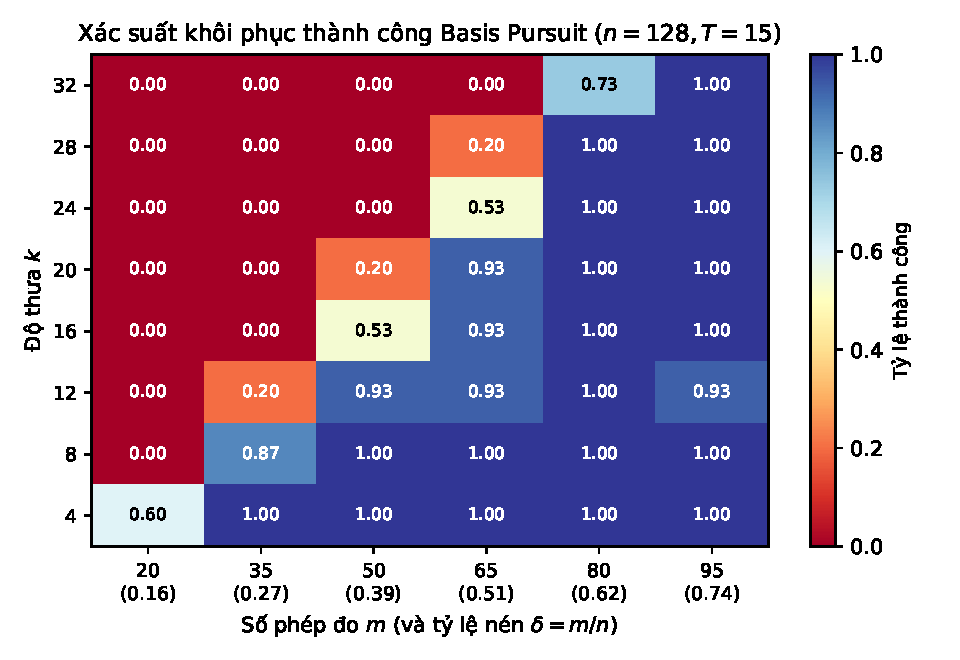
\includegraphics[width=0.82\textwidth]{fig_exp1_phase_transition.pdf}
    \caption{Biểu đồ nhiệt xác suất khôi phục thành công của Basis Pursuit (ADMM) theo $m$ và $k$ ($n = 128, T = 15$, \texttt{seed = 42}).}
    \label{fig:phase_transition}
\end{figure}

\subsection{Thí nghiệm 2: Khảo sát ảnh hưởng của nhiễu và tinh chỉnh tham số $\lambda$}
\textbf{Mục tiêu:} Kiểm chứng chặn sai số ổn định $\|\widehat{x} - x^\natural\|_2 \le C_1 \varepsilon$ và khảo sát đường cong đánh đổi giữa độ khớp dữ liệu và mức độ thưa theo tham số phạt $\lambda$ trong LASSO.

\textbf{Thiết lập tham số và kết quả thực nghiệm:}
\begin{itemize}
    \item Cố định $n = 256, m = 100, k = 12$, nhiễu trắng Gaussian theo 4 mức $\mathrm{SNR} \in \{10, 20, 30, 40\}\text{ dB}$, quét $\lambda$ trên 25 điểm logarit trong $[10^{-4}, 10^0]$ bằng FISTA.
    \item \textbf{Kết quả số thu được:}
    \begin{itemize}
        \item $\mathrm{SNR} = 10\text{ dB}$: $\lambda^* = 2{,}154 \times 10^{-1}$, sai số tương đối nhỏ nhất $\mathrm{RelErr}_{\min} = 0{,}3250$.
        \item $\mathrm{SNR} = 20\text{ dB}$: $\lambda^* = 4{,}642 \times 10^{-2}$, $\mathrm{RelErr}_{\min} = 0{,}1010$.
        \item $\mathrm{SNR} = 30\text{ dB}$: $\lambda^* = 1{,}468 \times 10^{-2}$, $\mathrm{RelErr}_{\min} = 0{,}0314$.
        \item $\mathrm{SNR} = 40\text{ dB}$: $\lambda^* = 4{,}642 \times 10^{-3}$, $\mathrm{RelErr}_{\min} = 0{,}0092$.
    \end{itemize}
    \item Sai số tối ưu giảm theo đúng tỷ lệ $\sqrt{10} \approx 3{,}16$ lần mỗi khi $\mathrm{SNR}$ tăng $10\text{ dB}$, khẳng định tính ổn định tuyến tính theo biên độ nhiễu. Hình \ref{fig:noise_lambda} và Hình \ref{fig:signal_recovery_stem} trình bày kết quả đồ thị thu được.
\end{itemize}

\begin{figure}[htbp]
    \centering
    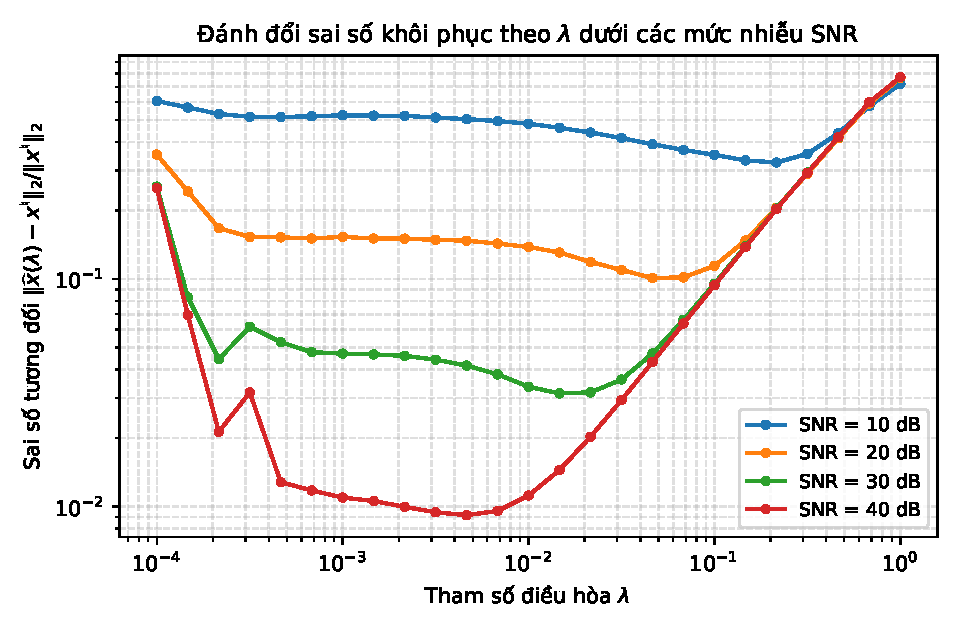
\includegraphics[width=0.80\textwidth]{fig_exp2_noise_lambda.pdf}
    \caption{Đường cong đánh đổi sai số tương đối theo tham số $\lambda$ dưới các mức nhiễu SNR khác nhau.}
    \label{fig:noise_lambda}
\end{figure}

\begin{figure}[htbp]
    \centering
    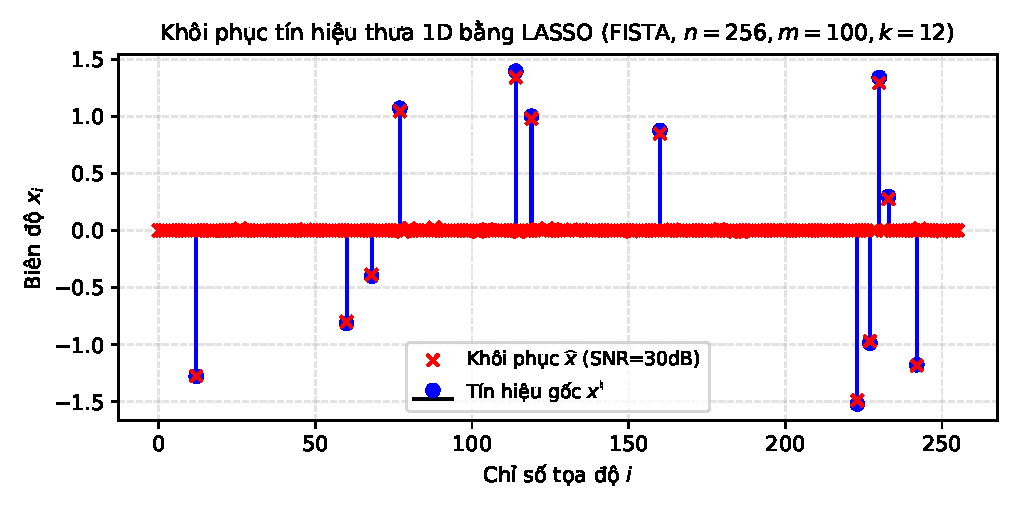
\includegraphics[width=0.86\textwidth]{fig_exp2_stem_1d.pdf}
    \caption{Kết quả khôi phục tín hiệu thưa 1D thực tế tại $\mathrm{SNR} = 30\text{ dB}$ ($n = 256, m = 100, k = 12$): Vị trí và biên độ xung khôi phục $\widehat{x}$ khớp chính xác với tín hiệu gốc $x^\natural$.}
    \label{fig:signal_recovery_stem}
\end{figure}

\subsection{Thí nghiệm 3: So sánh hiệu năng hội tụ giữa ISTA và FISTA}
\textbf{Mục tiêu:} Kiểm chứng bằng thực nghiệm tốc độ hội tụ lý thuyết $\mathcal{O}(1/k)$ của ISTA so với $\mathcal{O}(1/k^2)$ của FISTA.

\textbf{Thiết lập tham số và kết quả thực nghiệm:}
\begin{itemize}
    \item Bài toán LASSO với $n = 512, m = 120, k = 22$, $\sigma = 0{,}01$, $\lambda = 0{,}01 \|A^T b\|_\infty$; hằng số Lipschitz $L$ tính bằng Power Iteration; giá trị tham chiếu $F^* = 0{,}414618$ tính bằng 3.000 vòng lặp FISTA.
    \item \textbf{Kết quả sau 300 vòng lặp:} ISTA đạt $F(x^{300}) - F^* = 6{,}880 \times 10^{-2}$ (thời gian CPU $4{,}25\text{ ms}$), trong khi FISTA đạt $F(x^{300}) - F^* = 2{,}012 \times 10^{-6}$ (thời gian CPU $4{,}79\text{ ms}$) --- cải thiện độ chính xác hơn \textbf{30.000 lần} với chi phí tính toán gần như tương đương (Hình \ref{fig:convergence_comparison}).
\end{itemize}

\begin{figure}[htbp]
    \centering
    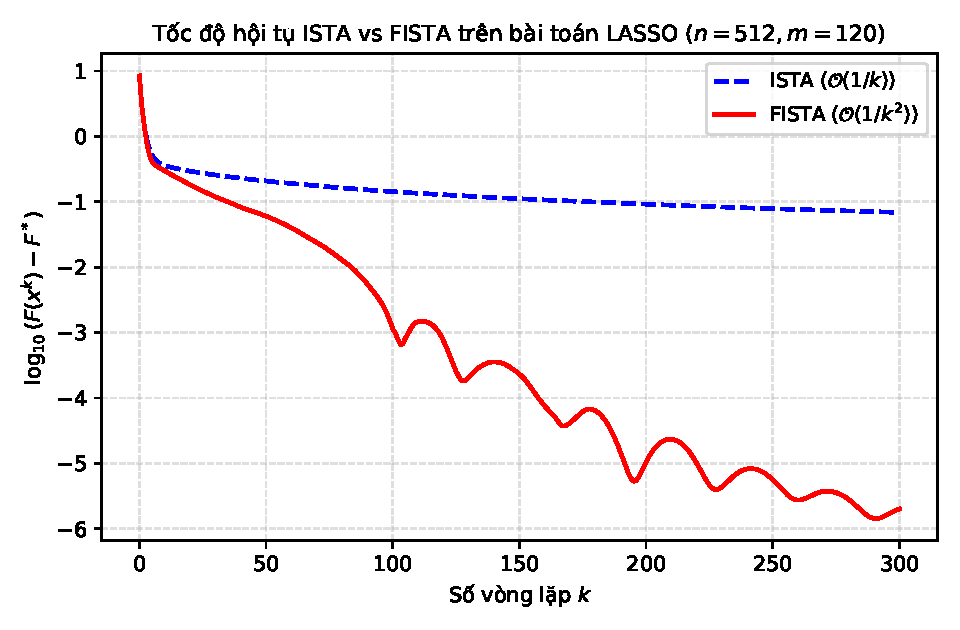
\includegraphics[width=0.80\textwidth]{fig_exp3_ista_vs_fista.pdf}
    \caption{Đồ thị thực nghiệm so sánh tốc độ suy giảm hàm mục tiêu $\log_{10}(F(x^k) - F^*)$ giữa ISTA và FISTA.}
    \label{fig:convergence_comparison}
\end{figure}

\subsection{Thí nghiệm 4: Khảo sát ảnh hưởng của Mutual Coherence}
\textbf{Mục tiêu:} Minh họa kết luận lý thuyết: ma trận có các cột tương quan cao (coherence lớn) sẽ làm suy giảm nghiêm trọng khả năng phục hồi của chuẩn $\ell_1$.

\textbf{Thiết lập tham số và kết quả thực nghiệm:}
\begin{itemize}
    \item Với $m = 80, n = 160, k = 8$ ($T = 25$ lần thử): Ma trận Gaussian độc lập $A$ có $\mu(A) = 0{,}4338$; ma trận $B$ được tạo bằng cách gán cột thứ hai $b_2 = b_1 + \delta$ với $\normtwo{\delta} = 10^{-3}$ rồi chuẩn hóa, cho $\mu(B) \approx 1{,}000000$.
    \item \textbf{Kết quả ghi nhận (Hình \ref{fig:coherence_impact}):} Ma trận $A$ khôi phục thành công $100{,}0\%$. Với ma trận $B$, khi tập hỗ trợ chứa cột $1$ (tương quan cao với cột $2$), tỷ lệ thành công sụt giảm mạnh xuống chỉ còn $16{,}0\%$; ngược lại, khi tập hỗ trợ tránh cặp cột $\{1, 2\}$, tỷ lệ thành công vẫn duy trì $100{,}0\%$.
\end{itemize}

\begin{figure}[htbp]
    \centering
    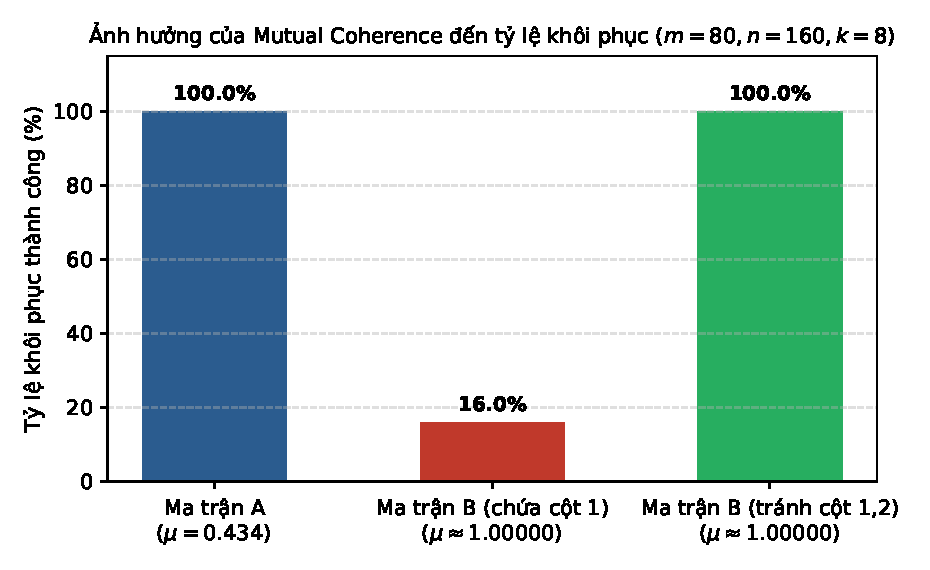
\includegraphics[width=0.78\textwidth]{fig_exp4_coherence.pdf}
    \caption{So sánh tỷ lệ khôi phục thành công của Basis Pursuit trên ma trận coherence thấp ($A$) và ma trận có cặp cột tương quan cao ($B$).}
    \label{fig:coherence_impact}
\end{figure}

\subsection{Thí nghiệm 5: Nén và tái tạo ảnh 2D với biến đổi Wavelet 2D}
\textbf{Mục tiêu:} Đánh giá khả năng ứng dụng thực tiễn của Lấy mẫu nén trên dữ liệu ảnh 2D (thưa xấp xỉ trong miền Wavelet \texttt{db4} mức 3) \cite{nguyen2016khoiphuc}.

\begin{figure}[htbp]
    \centering
    \begin{tikzpicture}[>=stealth, auto, scale=0.92, every node/.style={scale=0.92},
        block/.style={rectangle, draw=blue!80!black, fill=blue!8, thick, rounded corners, minimum height=2.8em, minimum width=5.6em, align=center, font=\footnotesize}]
        
        \node [block] (img) {Ảnh xám gốc\\$x \in \R^{p \times q}$};
        \node [block, right=1.1cm of img] (dwt) {Biến đổi Wavelet 2D\\$\theta = \Psi^T x$ (Thưa)};
        \node [block, right=1.1cm of dwt] (measure) {Đo nén ngẫu nhiên\\$b = A x = A\Psi \theta \in \R^m$};
        
        \node [block, below=1.3cm of measure] (recon) {Thuật toán lồi\\FISTA / ADMM};
        \node [block, left=1.1cm of recon] (idwt) {Wavelet ngược\\$\widehat{x} = \Psi \widehat{\theta}$};
        \node [block, left=1.1cm of idwt] (out) {Ảnh khôi phục\\$\widehat{x}$ ($\mathrm{SSIM} = 0{,}972$)};
        
        \draw [->, thick] (img) -- node [above] {\scriptsize Thưa hóa} (dwt);
        \draw [->, thick] (dwt) -- node [above] {\scriptsize $m \ll n$} (measure);
        \draw [->, thick] (measure) -- node [right] {\scriptsize Dữ liệu $b$} (recon);
        \draw [->, thick] (recon) -- node [above] {\scriptsize Hệ số $\widehat{\theta}$} (idwt);
        \draw [->, thick] (idwt) -- node [above] {\scriptsize Tái tạo ảnh} (out);
    \end{tikzpicture}
    \caption{Sơ đồ khối quy trình nén và tái tạo ảnh xám 2D sử dụng cơ sở biến đổi Wavelet và thuật toán tối ưu hóa lồi.}
    \label{fig:wavelet_cs_pipeline}
\end{figure}

\textbf{Thiết lập tham số và kết quả thực nghiệm:}
\begin{itemize}
    \item Sử dụng ảnh phantom hình học $64 \times 64$ ($n = 4096$ pixel), biến đổi Wavelet Daubechies 4 (\texttt{db4}) mức 3 làm cơ sở $\Psi$, thực hiện $m = 0{,}3n = 1228$ và $m = 0{,}5n = 2048$ phép đo ngẫu nhiên Gaussian và giải bằng 250 vòng lặp FISTA.
    \item \textbf{Kết quả định lượng thực tế (Hình \ref{fig:image_cs_result}):}
    \begin{itemize}
        \item Tại tỷ lệ đo $30\%$ ($m = 0{,}3n$): $\mathrm{PSNR} = 17{,}38\text{ dB}$, $\mathrm{SSIM} = 0{,}869$.
        \item Tại tỷ lệ đo $50\%$ ($m = 0{,}5n$): $\mathrm{PSNR} = 23{,}57\text{ dB}$, $\mathrm{SSIM} = 0{,}972$, tái tạo sắc nét toàn bộ cấu trúc biên và vùng ảnh.
    \end{itemize}
\end{itemize}

\begin{figure}[htbp]
    \centering
    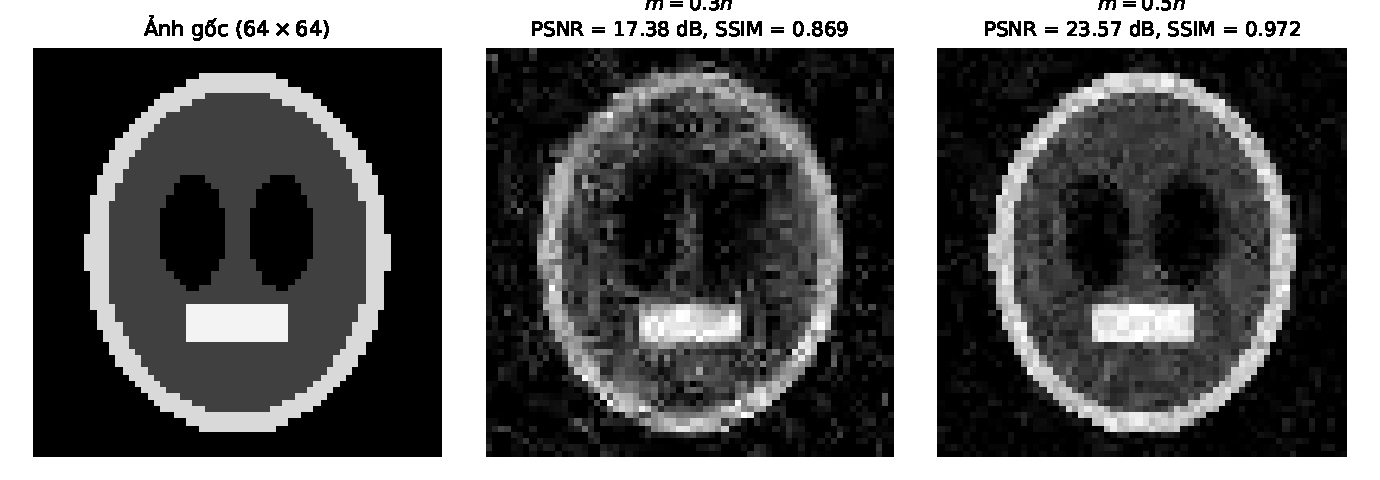
\includegraphics[width=0.95\textwidth]{fig_exp5_image_cs.pdf}
    \caption{Kết quả tái tạo ảnh 2D thực tế bằng FISTA trong miền Wavelet \texttt{db4} tại các tỷ lệ đo $m = 0{,}3n$ và $m = 0{,}5n$.}
    \label{fig:image_cs_result}
\end{figure}

\clearpage

% ==============================================================================
\section{Hệ thống câu hỏi tự kiểm tra và lời giải chi tiết}
\label{sec:cau_hoi_tu_kiem_tra}
% ==============================================================================
Phần này giải quyết trọn vẹn 8 câu hỏi cốt lõi được quy định trong hướng dẫn đề tài, đóng vai trò tự đánh giá mức độ thấu hiểu bản chất toán học từ lý thuyết đến cài đặt thuật toán.

\begin{exercise}[Bài 1: Tính lồi của chuẩn $\ell_1$ và tính không lồi của hàm đếm $\ell_0$]
Chứng minh tính lồi của chuẩn $\normone{x}$ và tính không lồi của đại lượng đếm $\normzero{x}$.
\end{exercise}

\begin{proof}[Lời giải chi tiết]
1. \textbf{Chứng minh chuẩn $\normone{x}$ là hàm lồi trên $\R^n$:}
Theo định nghĩa, hàm $f : \R^n \to \R$ là hàm lồi nếu với mọi $x, y \in \R^n$ và mọi hệ số $\alpha \in [0, 1]$, ta có $f(\alpha x + (1 - \alpha) y) \le \alpha f(x) + (1 - \alpha) f(y)$.
Áp dụng cho chuẩn $\ell_1$:
\[
\normone{\alpha x + (1 - \alpha) y} = \sum_{i=1}^n |\alpha x_i + (1 - \alpha) y_i|.
\]
Với mỗi tọa độ $i \in \{1, \dots, n\}$, sử dụng bất đẳng thức tam giác và tính chất không âm của $\alpha, 1 - \alpha$:
\[
|\alpha x_i + (1 - \alpha) y_i| \le |\alpha x_i| + |(1 - \alpha) y_i| = \alpha |x_i| + (1 - \alpha) |y_i|.
\]
Lấy tổng cả hai vế từ $i = 1$ đến $n$:
\[
\sum_{i=1}^n |\alpha x_i + (1 - \alpha) y_i| \le \alpha \sum_{i=1}^n |x_i| + (1 - \alpha) \sum_{i=1}^n |y_i| = \alpha \normone{x} + (1 - \alpha) \normone{y}.
\]
Điều này chứng minh $\normone{x}$ là hàm lồi trên $\R^n$.

2. \textbf{Chứng minh đại lượng $\normzero{x}$ không phải là hàm lồi:}
Ta chỉ ra một phản ví dụ cụ thể trong $\R^2$. Chọn hai vector $1$-thưa:
\[
x = (2, 0)^T \implies \normzero{x} = 1, \qquad y = (0, 2)^T \implies \normzero{y} = 1.
\]
Lấy hệ số $\alpha = 0.5 \in [0, 1]$, khi đó tổ hợp lồi giữa $x$ và $y$ là:
\[
z = 0.5 x + 0.5 y = (1, 1)^T \implies \normzero{z} = 2.
\]
Trong khi đó, vế phải của bất đẳng thức lồi cho:
\[
\alpha \normzero{x} + (1 - \alpha) \normzero{y} = 0.5(1) + 0.5(1) = 1.
\]
Vì $\normzero{z} = 2 > 1 = \alpha \normzero{x} + (1 - \alpha) \normzero{y}$, bất đẳng thức lồi bị vi phạm. Do đó $\normzero{x}$ không phải là hàm lồi.
\end{proof}

\begin{exercise}[Bài 2: Khôi phục tín hiệu thưa khi số phương trình ít hơn số ẩn ($m < n$)]
Tại sao hệ phương trình tuyến tính $Ax = b$ với $m < n$ vốn có vô số nghiệm lại có thể khôi phục duy nhất tín hiệu ban đầu nếu có thông tin thưa?
\end{exercise}

\begin{proof}[Lời giải chi tiết]
Trong đại số tuyến tính thông thường, nếu $A \in \R^{m \times n}$ với $m < n$, không gian hạt nhân $\ker(A)$ có số chiều ít nhất là $n - m \ge 1$. Do đó, tập nghiệm của hệ $Ax = b$ là một không gian affine $x_0 + \ker(A)$ có vô số phần tử trải dài trên toàn bộ không gian $\R^n$.

Tuy nhiên, tập hợp tất cả các vector $k$-thưa:
\[
\Sigma_k \coloneqq \{x \in \R^n : \normzero{x} \le k\} = \bigcup_{|S| \le k} \{x \in \R^n : \supp(x) \subseteq S\}
\]
không phải là một không gian vector mà là \textbf{hợp của $\binom{n}{k}$ không gian con $k$ chiều}. 
Khi ma trận $A$ thỏa mãn điều kiện cách ly (cụ thể là $\spark(A) > 2k$), không tồn tại bất kỳ vector khác không nào thuộc $\ker(A)$ mà có số tọa độ khác không $\le 2k$. 

Giả sử hệ có hai nghiệm $k$-thưa phân biệt $x, z \in \Sigma_k$ thỏa $Ax = Az = b$. Khi đó hiệu $h = x - z \in \ker(A)$ và thỏa mãn $\normzero{h} = \normzero{x - z} \le \normzero{x} + \normzero{z} \le 2k$. Do $\spark(A) > 2k$, điều này buộc $h = 0 \implies x = z$. 
Như vậy, không gian affine nghiệm $x_0 + \ker(A)$ chỉ cắt tập hợp $\Sigma_k$ tại \textbf{đúng một điểm duy nhất}, loại bỏ hoàn toàn vô số nghiệm không thưa còn lại.
\end{proof}

\begin{exercise}[Bài 3: Phân biệt Spark, NSP và RIP bằng một câu định nghĩa]
Phân biệt sự khác nhau căn bản giữa ba khái niệm trụ cột: Spark, NSP và RIP bằng đúng một câu cho mỗi khái niệm.
\end{exercise}

\begin{proof}[Lời giải chi tiết]
\begin{enumerate}
    \item \textbf{Spark:} Là số lượng cột phụ thuộc tuyến tính nhỏ nhất của ma trận đo $A$, đóng vai trò xác lập điều kiện cần và đủ hình học để nghiệm $k$-thưa là \emph{duy nhất} trong lớp các vector thưa.
    \item \textbf{NSP (Null Space Property):} Là điều kiện phân bố năng lượng chuẩn $\ell_1$ của không gian hạt nhân $\ker(A)$ ra bên ngoài tập hỗ trợ, đóng vai trò là điều kiện cần và đủ để \emph{thuật toán tối ưu lồi Basis Pursuit} tìm ra chính xác nghiệm nguyên bản.
    \item \textbf{RIP (Restricted Isometry Property):} Là tính chất ma trận đo gần như bảo toàn khoảng cách và độ dài Euclid trên tập hợp các vector thưa, đóng vai trò cung cấp công cụ định lượng bảo đảm tính \emph{ổn định bền vững khi phép đo bị ô nhiễm bởi nhiễu}.
\end{enumerate}
\end{proof}

\begin{exercise}[Bài 4: Chứng minh NSP đủ để Basis Pursuit khôi phục chính xác tín hiệu thưa]
Chứng minh tính chất không gian hạt nhân (NSP) bậc $k$ đủ để Basis Pursuit khôi phục đúng mọi vector $k$-thưa.
\end{exercise}

\begin{proof}[Lời giải chi tiết]
Cho $x^\natural \in \R^n$ là vector $k$-thưa tùy ý với tập hỗ trợ $S = \supp(x^\natural)$, thỏa mãn $|S| \le k$ và $x^\natural_{S^c} = 0$. Xét một nghiệm khả thi bất kỳ $x \ne x^\natural$ thỏa mãn hệ phương trình đo $Ax = b$. 
Đặt vector sai số $h \coloneqq x - x^\natural$. Rõ ràng $h \ne 0$ và:
\[
Ah = A(x - x^\natural) = b - b = 0 \implies h \in \ker(A) \setminus \{0\}.
\]
Ta phân tích chuẩn $\ell_1$ của $x = x^\natural + h$ theo hai tập chỉ số rời nhau $S$ và $S^c$:
\[
\normone{x} = \normone{x^\natural_S + h_S} + \normone{x^\natural_{S^c} + h_{S^c}}.
\]
Vì $x^\natural_{S^c} = 0$, ta có:
\[
\normone{x} = \normone{x^\natural_S + h_S} + \normone{h_{S^c}}.
\]
Sử dụng bất đẳng thức tam giác ngược: $\normone{x^\natural_S + h_S} \ge \normone{x^\natural_S} - \normone{h_S}$. Do đó:
\[
\normone{x} \ge \normone{x^\natural_S} - \normone{h_S} + \normone{h_{S^c}} = \normone{x^\natural} + (\normone{h_{S^c}} - \normone{h_S}).
\]
Do ma trận $A$ thỏa mãn tính chất NSP bậc $k$ và $h \in \ker(A) \setminus \{0\}$ với $|S| \le k$, theo định nghĩa NSP ta có $\normone{h_S} < \normone{h_{S^c}}$, dẫn đến:
\[
\normone{h_{S^c}} - \normone{h_S} > 0.
\]
Suy ra:
\[
\normone{x} > \normone{x^\natural}.
\]
Vì mọi nghiệm khả thi $x$ khác $x^\natural$ đều có chuẩn $\ell_1$ thực sự lớn hơn $\normone{x^\natural}$, tín hiệu gốc $x^\natural$ là nghiệm cực tiểu duy nhất của bài toán Basis Pursuit.
\end{proof}

\begin{exercise}[Bài 5: Cơ chế triệt tiêu hệ số $|a_i^T r^*| < \lambda \implies x_i^* = 0$ trong LASSO]
Giải thích tại sao điều kiện tương quan $|a_i^T r^*| < \lambda$ buộc tọa độ thứ $i$ của nghiệm LASSO phải bằng 0 chính xác.
\end{exercise}

\begin{proof}[Lời giải chi tiết]
Bài toán LASSO cực tiểu hóa hàm lồi $F(x) = \frac{1}{2}\normtwo{Ax - b}^2 + \lambda \normone{x}$. 
Điều kiện tối ưu KKT cần và đủ là $0 \in \partial F(x^*)$, tức:
\[
A^T(Ax^* - b) + \lambda \partial \normone{x^*} \ni 0 \iff A^T(b - Ax^*) \in \lambda \partial \normone{x^*}.
\]
Đặt vector phần dư tại nghiệm tối ưu là $r^* = b - Ax^* \in \R^m$. Khi đó $A^T r^* \in \lambda \partial \normone{x^*}$. 
Do chuẩn $\ell_1$ phân tách theo từng tọa độ, xét thành phần thứ $i$:
\[
a_i^T r^* \in \lambda \partial |x_i^*|,
\]
trong đó $a_i$ là cột thứ $i$ của ma trận $A$, và $\partial |x_i^*|$ là dưới vi phân của hàm trị tuyệt đối tại điểm $x_i^*$:
\[
\partial |x_i^*| = 
\begin{cases}
\{\sign(x_i^*)\}, & \text{nếu } x_i^* \ne 0, \\
[-1, 1], & \text{nếu } x_i^* = 0.
\end{cases}
\]
Giả sử phản chứng rằng $x_i^* \ne 0$. Khi đó $\partial |x_i^*| = \{\sign(x_i^*)\}$ với $\sign(x_i^*) \in \{-1, 1\}$, dẫn đến:
\[
a_i^T r^* = \lambda \cdot \sign(x_i^*) \implies |a_i^T r^*| = \lambda |\sign(x_i^*)| = \lambda.
\]
Sử dụng mệnh đề phản đảo: nếu $|a_i^T r^*| \ne \lambda$ (cụ thể là $|a_i^T r^*| < \lambda$), thì giả thiết $x_i^* \ne 0$ không thể xảy ra. Do đó bắt buộc:
\[
x_i^* = 0.
\]
Điều này chứng minh về mặt giải tích rằng tham số $\lambda$ hoạt động như một bộ lọc ngưỡng: chỉ những biến số có mức tương quan giữa cột đo $a_i$ và phần dư $r^*$ đạt đúng giá trị cực đại $\lambda$ mới được phép mang giá trị khác không.
\end{proof}

\begin{exercise}[Bài 6: Chứng minh công thức toán tử co ngưỡng mềm từ dưới vi phân]
Xuất phát từ định nghĩa dưới vi phân bậc nhất, hãy suy ra công thức toán tử co ngưỡng mềm $\mathcal{S}_t(v)$.
\end{exercise}

\begin{proof}[Lời giải chi tiết]
Toán tử co ngưỡng mềm $\mathcal{S}_t(v)$ giải bài toán tối ưu lồi ngặt 1 chiều:
\[
x^* = \argmin_{x \in \R} \phi(x), \quad \text{với } \phi(x) \coloneqq \frac{1}{2} (x - v)^2 + t |x|, \quad (t > 0).
\]
Vì $\phi(x)$ là hàm lồi ngặt liên tục, nghiệm $x^*$ tồn tại và duy nhất, xác định bởi điều kiện Fermat suy rộng:
\[
0 \in \partial \phi(x^*) \iff 0 \in (x^* - v) + t \partial |x^*| \iff v - x^* \in t \partial |x^*|.
\]
Ta xét ba trường hợp của điểm $x^*$:
\begin{enumerate}
    \item \textbf{Trường hợp 1 ($x^* > 0$):} Khi đó $\partial |x^*| = \{1\}$, điều kiện trở thành:
    \[
    v - x^* = t \implies x^* = v - t.
    \]
    Để điều kiện $x^* > 0$ được thỏa mãn, ta cần $v - t > 0 \iff v > t$.
    
    \item \textbf{Trường hợp 2 ($x^* < 0$):} Khi đó $\partial |x^*| = \{-1\}$, điều kiện trở thành:
    \[
    v - x^* = -t \implies x^* = v + t.
    \]
    Để điều kiện $x^* < 0$ được thỏa mãn, ta cần $v + t < 0 \iff v < -t$.
    
    \item \textbf{Trường hợp 3 ($x^* = 0$):} Khi đó $\partial |x^*| = [-1, 1]$, điều kiện trở thành:
    \[
    v - 0 \in t [-1, 1] \iff v \in [-t, t] \iff |v| \le t.
    \]
\end{enumerate}
Hợp nhất cả ba trường hợp lại, ta thu được nghiệm đóng tường minh:
\[
x^* = \mathcal{S}_t(v) = 
\begin{cases}
v - t, & \text{nếu } v > t, \\
0, & \text{nếu } |v| \le t, \\
v + t, & \text{nếu } v < -t,
\end{cases}
= \sign(v) \max(|v| - t, 0).
\]
\end{proof}

\begin{exercise}[Bài 7: Tại sao cần so sánh theo thời gian chạy thực tế thay vì chỉ đếm số vòng lặp?]
Nêu lý do khoa học tại sao khi đánh giá các thuật toán số, việc đo thời gian thực thi (CPU time) lại quan trọng hơn chỉ đếm số lượng vòng lặp.
\end{exercise}

\begin{proof}[Lời giải chi tiết]
Trong phân tích thuật toán tối ưu hóa, chi phí tính toán của một lần lặp phụ thuộc hoàn toàn vào cấu trúc của bài toán con tại mỗi bước:
\begin{itemize}
    \item \textbf{Các thuật toán bậc nhất (ISTA, FISTA):} Mỗi vòng lặp chỉ đòi hỏi hai phép nhân ma trận--vector $Ax$ và $A^T r$ cùng phép co ngưỡng mềm $\mathcal{S}_t(\cdot)$ với chi phí tính toán rất thấp $\mathcal{O}(mn)$.
    \item \textbf{Các phương pháp bậc hai và điểm trong (Interior Point, Newton):} Có tốc độ hội tụ bậc hai tiệm cận và thường hội tụ trong rất ít vòng lặp (chỉ $15 - 30$ vòng lặp). Tuy nhiên, tại mỗi vòng lặp, phương pháp này đòi hỏi phải thiết lập và giải hệ phương trình tuyến tính kích thước $m \times m$ (hệ Newton) hoặc nghịch đảo ma trận, tiêu tốn chi phí $\mathcal{O}(m^3 + m^2n)$ và bộ nhớ khổng lồ.
\end{itemize}
Do đó, nếu chỉ so sánh số vòng lặp, người nghiên cứu sẽ lầm tưởng các thuật toán điểm trong hiệu quả hơn. Trên thực tế với dữ liệu lớn ($n \ge 10^5$), thời gian chạy một vòng lặp điểm trong có thể lâu hơn hàng nghìn vòng lặp của FISTA. Thời gian thực thi CPU phản ánh chân thực chi phí tài nguyên và khả năng mở rộng của thuật toán trong môi trường thực nghiệm.
\end{proof}

\begin{exercise}[Bài 8: Tại sao khi có nhiễu, khôi phục chính xác tuyệt đối không còn là mục tiêu hợp lý?]
Khi dữ liệu đo bị ô nhiễm bởi nhiễu, vì sao mục tiêu khôi phục chính xác tuyệt đối ($\widehat{x} = x^\natural$) không còn khả thi và hợp lý về mặt toán học?
\end{exercise}

\begin{proof}[Lời giải chi tiết]
Xét mô hình đo có nhiễu: $b = A x^\natural + e$ với $e \ne 0$. 
Không gian con sinh bởi $k$ cột tương ứng với tập hỗ trợ thực tế $S = \supp(x^\natural)$ là $\mathcal{R}(A_S) = \{A_S z : z \in \R^k\}$. Vì vector nhiễu $e \in \R^m$ mang tính ngẫu nhiên (ví dụ nhiễu Gaussian), vector quan sát $b = A_S x^\natural_S + e$ hầu như chắc chắn \textbf{không nằm trong không gian con $\mathcal{R}(A_S)$}.

Nếu một thuật toán cố tình ép buộc khôi phục chính xác hệ thức đẳng thức $Ax = b$, thuật toán sẽ buộc phải huy động thêm các cột đo nằm ngoài tập hỗ trợ thực tế ($j \notin S$) để cố gắng khớp phần năng lượng của vector nhiễu $e$. Hiện tượng này gây ra lỗi \textbf{quá khớp nhiễu} (\emph{noise overfitting}), làm sai lệch hoàn toàn tập hỗ trợ và khiến vector khôi phục không còn thưa.

Do đó, mục tiêu toán học đúng đắn khi có nhiễu là \textbf{khôi phục ổn định} (\emph{stable recovery}): chấp nhận sai số tái tạo và kiểm soát sai số này bị chặn tuyến tính theo biên độ năng lượng của nhiễu:
\[
\normtwo{\widehat{x} - x^\natural} \le C_0 \frac{\sigma_k(x^\natural)_1}{\sqrt{k}} + C_1 \normtwo{e}.
\]
Khi biên độ nhiễu tiến về 0 ($\normtwo{e} \to 0$), sai số khôi phục sẽ tiến về 0, bảo đảm tính liên tục và độ bền vững của mô hình.
\end{proof}


% Kết luận và hướng phát triển
% ==============================================================================
% KẾT LUẬN VÀ HƯỚNG PHÁT TRIỂN
% ==============================================================================
\chapter*{Kết luận và hướng phát triển}
\addcontentsline{toc}{chapter}{Kết luận và hướng phát triển}

\section*{Tổng kết đề tài}
Đồ án đã nghiên cứu có hệ thống bài toán khôi phục tín hiệu thưa bằng cực tiểu hóa chuẩn $\ell_1$, làm sáng tỏ câu trả lời cho \textbf{ba câu hỏi cốt lõi}:
\begin{enumerate}
    \setlength{\itemsep}{2pt}\setlength{\parskip}{0pt}
    \item \textbf{Tín hiệu có được xác định duy nhất không?} Điều kiện $\spark(A) > 2k$ xác lập ranh giới cần và đủ cho tính duy nhất trong lớp vector $k$-thưa, đòi hỏi số phép đo tối thiểu $m \ge 2k$.
    \item \textbf{Thuật toán tối ưu lồi có tìm được nghiệm không?} Tính chất không gian hạt nhân (NSP) bậc $k$ là điều kiện cần và đủ để Basis Pursuit tìm đúng nghiệm gốc (vượt qua tính NP-hard của $\ell_0$), bên cạnh tiêu chuẩn đủ tính nhanh qua Mutual Coherence $\mu(A)$.
    \item \textbf{Kết quả có ổn định khi có nhiễu không?} Tính chất RIP ($\delta_{2k} < \sqrt{2} - 1$) bảo đảm nghiệm của BPDN/LASSO thỏa mãn chặn sai số bền vững $\normtwo{\widehat{x} - x^\natural} \le C_0 \frac{\sigma_k(x^\natural)_1}{\sqrt{k}} + C_1 \varepsilon$.
\end{enumerate}

Về mặt thuật toán, việc kết hợp toán tử co ngưỡng mềm với gia tốc Nesterov (FISTA, $\mathcal{O}(1/k^2)$), chiếu gradient (GPSR) và phân tách biến (ADMM) đã được kiểm chứng qua 5 kịch bản thực nghiệm số (chuyển pha, nhiễu SNR, hội tụ, coherence và tái tạo ảnh 2D Wavelet đạt $\mathrm{SSIM} = 0{,}972$).

\section*{Hướng phát triển mở rộng}
\begin{itemize}
    \setlength{\itemsep}{2pt}\setlength{\parskip}{0pt}
    \item \textbf{Tổng biến thiên (Total Variation - TV):} Khôi phục tín hiệu có gradient thưa, bảo tồn biên cạnh sắc nét trong ảnh y khoa và vệ tinh.
    \item \textbf{Tín hiệu thưa theo nhóm (Group Sparsity):} Khai thác cấu trúc hệ số thưa theo cụm bằng chuẩn hỗn hợp $\ell_{2,1}$.
    \item \textbf{Khôi phục ma trận hạng thấp (Matrix Completion):} Cực tiểu hóa chuẩn hạt nhân (\emph{Nuclear Norm}) cho bài toán ma trận suy biến thưa và tách nền video.
    \item \textbf{Deep Unfolding:} Nhúng các bước lặp FISTA/ADMM thành tầng mạng nơ-ron sâu (như LISTA) để học tham số tối ưu trực tiếp từ dữ liệu.
\end{itemize}

% ------------------------------------------------------------------------------
% 4. TÀI LIỆU THAM KHẢO (BACKMATTER)
% ------------------------------------------------------------------------------
\clearpage
\bibliographystyle{plain}
\bibliography{bibliography/references}
\addcontentsline{toc}{chapter}{Tài liệu tham khảo}

% ------------------------------------------------------------------------------
% 5. PHỤ LỤC (MÃ NGUỒN THỰC NGHIỆM)
% ------------------------------------------------------------------------------
\appendix
\renewcommand{\chaptertitlename}{Phụ lục}
% ==============================================================================
% PHỤ LỤC: MÃ NGUỒN THỰC NGHIỆM MÔ PHỎNG
% ==============================================================================
\chapter{Mã nguồn thực nghiệm mô phỏng}
\label{app:source_code}

Phụ lục này cung cấp toàn bộ mã nguồn Python độc lập được sử dụng để sinh dữ liệu, giải các bài toán tối ưu (ISTA, FISTA, ADMM) và vẽ trực tiếp 6 biểu đồ kết quả thực nghiệm trong Chương \ref{chap:thuc_nghiem}.

\section{Môi trường thực thi và kết quả đầu ra trên dòng lệnh}
\begin{itemize}
    \item \textbf{Môi trường:} Python 3.12+, thư viện \texttt{NumPy}, \texttt{Matplotlib}, \texttt{PyWavelets}.
    \item \textbf{Hạt giống ngẫu nhiên:} \texttt{SEED = 42} (\texttt{numpy.random.default\_rng(42)}).
    \item \textbf{Lệnh chạy:} \texttt{python code/run\_experiments.py} (thời gian chạy toàn bộ 5 thí nghiệm khoảng $10$ giây).
\end{itemize}

{\scriptsize
\begin{verbatim}
=== THÍ NGHIỆM 1: CHUYỂN PHA BASIS PURSUIT (ADMM) ===
k \ m |   20 |   35 |   50 |   65 |   80 |   95
-----------------------------------------------
    4 | 0.60 | 1.00 | 1.00 | 1.00 | 1.00 | 1.00
    8 | 0.00 | 0.87 | 1.00 | 1.00 | 1.00 | 1.00
   12 | 0.00 | 0.20 | 0.93 | 0.93 | 1.00 | 0.93
   16 | 0.00 | 0.00 | 0.53 | 0.93 | 1.00 | 1.00
   20 | 0.00 | 0.00 | 0.20 | 0.93 | 1.00 | 1.00
   24 | 0.00 | 0.00 | 0.00 | 0.53 | 1.00 | 1.00
   28 | 0.00 | 0.00 | 0.00 | 0.20 | 1.00 | 1.00
   32 | 0.00 | 0.00 | 0.00 | 0.00 | 0.73 | 1.00

=== THÍ NGHIỆM 2: ẢNH HƯỞNG NHIỄU VÀ THAM SỐ LAMBDA (LASSO) ===
SNR = 10 dB | lambda* = 2.1544e-01 | RelErr min = 3.2500e-01 | k_hat = 35
SNR = 20 dB | lambda* = 4.6416e-02 | RelErr min = 1.0095e-01 | k_hat = 48
SNR = 30 dB | lambda* = 1.4678e-02 | RelErr min = 3.1415e-02 | k_hat = 44
SNR = 40 dB | lambda* = 4.6416e-03 | RelErr min = 9.1608e-03 | k_hat = 37

=== THÍ NGHIỆM 3: SO SÁNH HỘI TỤ ISTA VS FISTA ===
F* = 0.414618
ISTA  (300 iters): F - F* = 6.880e-02, CPU time = 4.25 ms
FISTA (300 iters): F - F* = 2.012e-06, CPU time = 4.79 ms

=== THÍ NGHIỆM 4: ẢNH HƯỞNG CỦA MUTUAL COHERENCE ===
mu(A) = 0.4338 -> Tỷ lệ thành công: 100.0%
mu(B) = 1.000000 -> Hỗ trợ chứa cột 1: 16.0% | Tránh {1,2}: 100.0%

=== THÍ NGHIỆM 5: NÉN VÀ TÁI TẠO ẢNH 2D WAVELET DB4 ===
Tỷ lệ đo m/n = 0.3 (m = 1228/4096) -> PSNR = 17.38 dB, SSIM = 0.8687
Tỷ lệ đo m/n = 0.5 (m = 2048/4096) -> PSNR = 23.57 dB, SSIM = 0.9722
\end{verbatim}
}

\section{Toàn bộ mã nguồn chương trình (\texttt{code/run\_experiments.py})}
\lstinputlisting[caption={Mã nguồn Python thực nghiệm mô phỏng cho 5 kịch bản trong Chương 5.}]{code/run_experiments.py}


\end{document}
